%%
%z = FF+M
%kr = k*W/w
%%
%one = ( (z*(z+k))/(alpha*w*(z+kr)) )^gamma
%two = (gamma*FF/alpha/w) * ((z*(z+k))/(alpha*w*(z+kr)))^(gamma-1)
%thr = kr*(k-kr)/((z+kr)^2)
%
\newcommand{\kr}{ \frac{\kappa w_\infty}{w(a_s)} }
\newcommand{\one}{
        \left(\frac{Z(Z+\kappa)}{\alpha w(a_s)(Z+\kr)}\right)^\gamma
}
\newcommand{\two}{
        \left(\frac{\gamma F}{\alpha w(a_s)}\right) \left(\frac{Z(Z+\kappa)}{\alpha w(a_s)(Z+\kr)}\right)^{\gamma-1}
}
\newcommand{\thr}{
        \frac{\left(\kr\right)\left(\kappa-\kr\right)}{(Z+\kr)^2}
}
%
\newcommand{\oneA}{
        \left(\frac{Z^*(Z^*+\kappa)}{w(a_s)(Z^*+\kr)}\right)^\gamma
}
\newcommand{\twoA}{
        \left(\frac{\gamma F^*}{w(a_s)}\right) \left(\frac{Z^*(Z^*+\kappa)}{w(a_s)(Z^*+\kr)}\right)^{\gamma-1}
}
\newcommand{\thrA}{
        \frac{\left(\kr\right)\left(\kappa-\kr\right)}{(Z^*+\kr)^2}
}


%sugar

%\begin{itemize}
%\item sweep Intro, Methods, Results, 
%\item draft Discussion
%\item fix up Intro
%\item sweep for SPM vs. DDM vs. ASM
%\item sweep for fast, medium and slow growth
%\item emphasize relation to ASM
%\end{itemize}

%
\section{Introduction}

%
The simplified dynamics of SPMs capture a broad range of RP variation, however
RP behavior can be complicated by the inclusion of individual growth. %when model dynamics are elaborated by the inclusion of individual growth. 
%by While the SPM captures the majority of variation in RPs, models including 
%individual growth dynamics  also interact with the structure of productivity  
%to effect RPs.
%is the next most influential dynamic for explaining RP variation {\color{red}cite or generalize}. 
The SPM captures the net effect of biomass production by assuming all aspects 
of biomass production (i.e. maturity, recruitment, growth, etc.) are modeled by the %together in 
the production function. There are a number of %teasing apart?
approaches to model these dynamics to explicitly tease out these processes \cite{quinn_quantitative_1999, hilborn_quantitative_1992}, 
but for the purpose of stock assessment, when data limitations are not too severe, %in a {\color{red}``data-rich'' (not data-limited)} setting it is currently considered best 
%{\color{red}cite age structured model, selectivity models, any other model I can find (Munch, Bethany?)} 
age structured models, ASM, \cite{methot_stock_2013} are often considered best practice.
%%ice to use an age structured models (ASM) \cite{methot_stock_2013}. 

%Due to their complexity, cope_stock_2023
%ASMs require a lot of expensive data to make make inferences from. Even when these data do exists, 
%the highly parameterized structures used in these models introduce the potential for identifiability 
%issues {\color{red} cite}.

%{\color{red} citations below, ?change methot above?}
%
%{\color{red} tansition }

%
ASMs separate the dynamics of the population into cohorts moving between age 
classes through time. %of interrelated discrete %interrelated age classes. 
Cohorts are governed by a system of equations %similar ODEs 
such that each cohort is modeled in a way that resembles the SPM in time. By
tracking the average size, and relative contribution to production, of individuals %, and their relative contribution to production, %of individuals, in 
in the population as they age, ASMs inform models of individual growth. ASMs 
require the specification of many parametric forms for describing the recruitment, 
growth, maturity, selectivity, etc. that enmesh the system of equations at their 
core. These complex structures allow ASMs to capture a wide range of dynamics, however 
the simultaneous accurate specification, implementation, and estimation of all of 
these forms, and the parameters they imply, requires a lot of expensive data 
of many different types to fit. 
%they specifying the enmeshing ODE structures requires accurate 
%specification of many  
%models of individual growth to be informed 
%with spawning biomass determined by the $a-1^{th}$although with. 
%that resemble the structure of the SPM setting. the emesshing of ODES adds involves
%The dynamics of each cohort resemble that of the simplified SPM setting, however 
%as age classes grow through time the outputs from the $a^{th}$ age class becomes 
%the input for the $a+1^{th}$ age class  
%
%  allow for individual growth and maturity to be modeled as cohorts that age 
%through time.
%Modeling age and length/weight structure in the population allows for
%individual growth and maturity to be modeled as cohorts that age through time.
%Despite this added complexity, at their core ASMs rely on similar dynamics as
%seen in Eq. (\ref{ode}), however in ASMs the above ODE is expanded to a system
%of interrelated ODEs for each age class.

%%
%{\color{red}
%\begin{itemize}
%%\item what is an ASM (reiterate intro intro and maybe a bit more)
%%\item maybe introduce VB growth?
%%\item require a lot of expensive data
%\item ?? Even when these data do exists, the highly parameterized structures 
%used in these models introduce the potential for identifiability issues {\color{red} cite}.
%\item ?expensive to compute.?
%\end{itemize}
%}

%
Delay differential models, DDMs (or delay difference models in discrete time) 
are an intermediate approach between SPMs and ASMs. At their simplest, DDMs do 
not necessarily model individual growth \cite{dick_depletion-based_2011, aalto_separating_2015}, 
but still these models are beneficial in modeling the lag between egg production 
and recruitment into the reproducing population.  %\cite{dick_depletion-based_2011, aalto_separating_2015}.
%Simple DDMs may not explicitily model individual growth \cite{dick_depletion-based_2011, aalto_separating_2015} %{\color{red}cite EJ Alec and Aalto et al. 2015}, 
%but even so the delayed structure of DDMs are beneficial in modeling the lag between egg production 
%and recruitment into the reproducing population. 
%as well as the natural autocorrelation often observed with stock size.
By linking selectivity and maturity together with a simplified knife-edge lagged 
model, more complex DDMs are capable of exactly representing simple ASMs \cite{deriso_harvesting_1980, fournier_length-based_1987, schnute_general_1985, schnute_general_1987}. 
%with an %explicit and compact representation of simple individual growth and maturity dynamics.
%That said, DDMs are capable of explicitly representing simple individual growth and maturity dynamics 
%\cite{walters_continuous_2020}, \cite[pg. 334]{hilborn_quantitative_1992} \cite{Quinn and Deriso 1999}.
%
%NOTE: maybe establish maturity linked to selectivity here
When information about individual growth is available these DDMs have enough 
growth, lagged maturity, and lagged selectivity modeling infrastructure to make 
use of the information without requiring the use of heavily parameterized ASMs. %e.g. \cite{black rockfish assessment}.
%can put those data to use without the need to parameterize the full age at length table of a fully age stuctured model \cite{black rockfish assessment}.
%}
%DDMs that can tease out individual growth and maturity from recruitment to explain net production 
%as separate but interconnected processes {\color{red} cite schnute, deriso \cite{walters_continuous_2020}, \cite[pg. 334]{hilborn_quantitative_1992}, Quinn and Deriso 1999}
The relatively smaller size, and yet flexible dynamics, of DDMs makes them ideal for 
modeling ``data-limited'' stocks, while still entertaining varied hypotheses that 
relate growth and maturity.  
%When information about growth is available the DDM allows  may be known but not the full age at length table of an age stuctured model \cite{black rockfish assessment}

%%
%{\color{red}
%\begin{itemize}
%\item state the main point of this chapter.
%\item Tack on analytical RPs angle
%\item reiterate steps in this chapter.
%\end{itemize}
%}


%RPS
DDMs are effective and flexible data-limited models, however there use in 
stock assessments have been limited by the accessibility of RP calculations 
\cite{munyandorero_analytical_2023}. %{\color{red} add other paper? aalto?}. %While
%
This chapter expands the previous chapters' analyses of RP biases under the 
two-parameter BH model using the DDM outlined by Walters \cite{walters_continuous_2020}
to account for RP bias as individual growth and maturity dynamics vary.
%
The simulation design using this DDM requires a derivation 
of analytical RPs that account for individual growth and
maturity dynamics under a Schnute model of recruitment.
%%expressions that account for individual growth andmaturity dynamics
%%This chapter 
%expands on existing work to develop accessible DDM RPs \cite{dick_depletion-based_2011, munyandorero_analytical_2023},
%by deriving analytical RP expressions that account for individual growth and
%maturity dynamics, with the continuous time DDM outlined by Walters \cite{walters_continuous_2020}, 
%under a Schnute model of recruitment. 
%There has been some work to develop accessible RPs using DDMs \cite{dick_depletion-based_2011, munyandorero_analytical_2023}, 
%and this work expands on those efforts.
%Here the Schnute-Deriso delay-differential structure, as recently posed by Walters \cite{walters_continuous_2020}, %in a continuous time setting , is used 
%is considered with a Schnute model of recruitment to derive analytical DDM RP 
%expressions that account for individual growth maturity dynamics.
%{\color{red}
%this work expands those efforts by deriving and analytical DDM RP expressions under the Schnute model of recruitment. 
%Using the Schnute-Deriso delay-differential structure to include individual growth, as recently detailed by Walters \cite{walters_continuous_2020},
%under the Schnute modeled of recruitment.
%}
%This model under the DDM \cite{walters_continuous_2020} with individual growth, under the Schnute modeled of recruitment. 
Munyandorero \cite{munyandorero_analytical_2023} gives RP expressions using 
this same DDM %outlined by Walters 
under BH, Ricker, and Shepard recruitment. 
My work in this chapter adds to that work by deriving RP calculations under 
the Schnute model. The Munyandorero results are reiterated by the BH and Ricker 
model special cases of the Schnute DDM. % and reiterate the Munyandorero results; deriving these results under the 
The Schnute model further unifies these results with a single analytical form that 
also extends RP results to include Schaefer and Cushing-like models. 
%%} as additional special cases. 
%%%Furthmore the Schnute model unifies these models with a single analytical result. 
%%This study further {\color{red}reveils} that RPs are largely dtermined by the 
%%form of R. While growth does have an effect on RPs in these models, the effect 
%%is secondary to the form of R.
These analytical expressions form the basis of the simulation-based inquiry of 
RP biases as they are influenced by individual growth and maturity dynamics.
%under BH recruitment, and the DDM expands the metamodeling infustructure
%to understand how RP biases are influenced by individual growth and maturity dynamics. 
%% the metamodeling methodology to explore how RP estimation is  

%
These analytical expressions form the basis of the simulation-based inquiry of
RP biases under BH recruitment, when the data are generated broadly under the 
Schnute model. Additionally, the DDM setting allows for a probe into how recruitment and 
growth interact to effect RP estimation. 
%%
%The DDM delevoped here extends the analysis of how productivity model misspecification 
%can bias RPs estimation as individual growth and maturity dynamics are added to the model. 
%The DDM allows for a probe into how recruitment and growth interact to effect RP estimation.
%when in the presence of individual growth and maturity dynamics
%Models that include individual growth and maturity dynamics %which account for individual growth and age-structure
%are another important practical setting for extending the understanding of how
%productivity model misspecification can bias RPs estimation. 
This work begins with a derivation of RPs under the three-parameter Schnute 
DDM. Analytical RP calculations are then structured so as to fit into the 
simulation design methods presented in Section (\ref{sLHS}), and RP biases are 
then analyzed via the GP metamodel developed in Sections (\ref{gpmm}) and (\ref{sMeta}).
% as it is extended to the case of BH analysis in Section (\ref{sMeta}).


%{\color{red} Gotta introduce and discuss bias estimation
%
%In this study I consider the behavior of inference when index data are simulated
%from three-parameter PT and Schnute production models, but the simulated data are fit
%using intentionally misspecified two-parameter logistic or BH production models. The
%work begins with a derivation of RPs under the three-parameter models. A method is
%then presented for generating simulation designs based on the parametric form of RPs
%which serves as a control on the nature of simulated model misspecification. Finally a
%Gaussian Process (GP) metamodel [12] is constructed for exploration and analysis of biases.
%A key insight of this approach is that bias is considered broadly across RP-space to
%uncover patterns and correlations between RPs. The GP metamodel is explicit about
%trade-offs between RPs so as to inform the full utility of reducing bias, as well as to
%suggest mechanisms for understanding what causes bias. Further, the effect of contrast
%on estimation is considered together with model misspecification.
%
%%Additionally
%Models that include individual growth and maturity dynamics %which account for individual growth and age-structure
%are another important practical setting for extending the understanding of how
%productivity model misspecification can bias RPs estimation.
%% in stock 
%%assessment models is the context of dynamics which account for individual 
%%growth and age-structure.
%%which include individual growth in the population dynamics. 
%%It is also necessary to study RP bias in the context of
%%%An additional extension is to study of RP bias in the context of
%%individual growth and age-structure. %d models.
%%%A further important modeling extension is to include the dynamics of 
%%%age-structure in the population. 
%The Deriso-Schnute delay-difference (DD) model provides a compact
%representation of simple age-structured dynamics \shortcite{deriso_harvesting_1980, schnute_general_1985, schnute_general_1987}. %\color{red} cite equivalnece}. 
%While various modeling strategies may be considered for including effects of
%age-structure in the population, the Deriso-Schnute DD model presents an ideal
%model for the simulation setting presented here. The compact representation of
%the Deriso-Schnute DD model via delay-differential equations accounts for the
%effects of individual growth and maturity while maintaining relatively fast
%computation.  %while accounting for the effects of individual growth and maturity.  %and parsimonious parameterization of growth   for the simulation setting presented here.
%
%%
%The DD model is derived directly from an assumption of Von Bertalanffy growth \shortcite{von_bertalanffy_quantitative_1938} %{\color{red} cite } 
%in weight, as seen in Eq (\ref{vbGrowth}). In this setting Von Bertalanffy
%growth relates individual age to individual weight by assuming linear
%instantaneous growth (as parameterized by the growth parameters $\kappa$ and
%$w_\infty$). The DD model expands the idea of biomass production into the
%processes of recruitment, individual growth, and maturity. This formulation
%separates the number of individuals in the population ($N$) from the biomass
%of the population ($B$). The dynamics of $N$, as seen in Eq (\ref{nEq}), are
%very similar to that of the Deriso production model presented above, however
%the role of the production function is now filled by a "recruitment" function
%which describes how new individuals are added to the numbers equation. The $B$ dynamics,
%%of accounting for $B$, as seen in Eq(\ref{bEq}), %, described from left to right), 
%can then be seen to describe biomass by an account of 1) biomass of new
%recruits, 2) the net growth of existing biomass, and 3) biomass lost due to
%mortality. The model accounts for maturity as knife-edge maturity at the
%instant an individual reaches age $a_0$.
%%
%}


%RPs are largely determined by R, and to a much lesser effect growth.
%RP calculation have been elusive \cite{Munyandorero2023, Schnute}.
%MSY-based RPs (e.g., Aalto et al. 2015),
%\cite{Munyandorero2023} gives results for BH, Ricker, and three parameter Shepard.
%I give results for Schnute which includes BH, Ricker, Schafer, and Cushing as a a special case.
%
%
%%
%\begin{itemize}
%	\item[\checkmark] SPM describe productivity via net recruitment of biomass, natural mortality and fishing.
%	\item[\checkmark] ASM describe recruitment in numbers, indivual growth to biomass, natural mortality, fishing, and selectivity.
%	\item[\checkmark] selectivity requires a lot of data to parameterize and describe. 
%	\item[\checkmark] in a data poor setting, DDM offer an effective intermediate.
%	\item RPs are largely determined by R, and to a much lesser effect growth. 
%	\item growth is often estimated external to the dynamics model, although we will see that in certain situations an index can inform growth as well.
%\end{itemize}
%
%%
%\begin{itemize}
%	\item[\checkmark] intermediate in complexity between SPMs and ASMs. (Next step in complexity)
%	\item[\checkmark] perfect size model for data poor stocks, when some knowledge about growth may be known but not the full age at length table of an age stuctured model \cite{black rockfish assessment}
%	\item[\checkmark] These models include natural mortality, and may or may not \cite{dbSRA} incorporate individual (somatic) growth. 
%	\item 
%	\item time series fisheries data (catch, biomass and/or numbers)
%	\item delay structure naturally represents time from egg to recruitment, and the natural auto correlation of stock size with itself.
%	\item naturual mortaility
%	\item 
%	\item RP calculation have been elusive \cite{Munyandorero2023, Schnute}.
%	\begin{itemize}
%	\item \cite{Munyandorero2023} gives results for BH, Ricker, and three parameter Shepard
%	\item I give results for Schnute which includes BH, Ricker, Schafer, and Cushing as a a special case.
%	\end{itemize}
%	
%	\item data poor setting
%\end{itemize}
%
%
%%Munyandorero 2012, 2015, 2022, 2023*
%\begin{itemize}
%\item fitted to time series of fishery data
%\item received little attention in developing MSY-based RPs or proxies 2015, 2022
%\item intermediate in complexity between SPMs and ASMs.
%\item allows development of RPs. The unanimous answer was: “No;
%\item MSY-based RPs (e.g., Aalto et al. 2015),
%\item Relates:
%\begin{itemize}
%	\item lag: (i) to the number of years from egg deposition until the young fish become vulnerable to the fishery,
%	\item $B_{t-lag}$: (ii) to the fact that the exploitable stock size in any time step depends on stock sizes in previous time steps,
%\end{itemize}
%\item These models include natural mortality, individual growth
%\item that the populations’ recruit 
%\item adult components can be tuned by separate indices of abundance in number, weight, or both.
%\item (i) constant growth and mortality rates
%\item (ii) equal ages of knife-edge selectivity (i.e., recruitment to the fishery) and knife-edge maturity, implying that adults and recruits in the population are fully selected and have equal (full) reproductive capacity.
%\end{itemize}
%
%%DB-SRA
%\begin{itemize}
%\item 
%Management of “data-rich” stocks is often based on complex assessments that incorporate a variety of data sources and that provide estimates of stock status, various management targets or reference points, and sustainable yield. 
%There remain very many fish stocks for which data are too limited to support these data-rich approaches. 
%The focus of assessment for “data-poor” stocks is often restricted to estimates of sustainable yield because insufficient data are available to estimate the full suite of reference points. 
%Common approaches for data-poor stocks include defining a proxy value for sustainable catch ($F_msy$ proxy), e.g. recent average catch, which may be precautionarily reduced to account for uncertainty. 
%Advice regarding the extent of these reductions has been based on qualitative descriptions of stock status, such as “above Bmsy” or “overfished” (Restrepo et al., 1998).
%\item data poor model with lots of flexibility and RPs
%\item no individual growth
%\end{itemize}
%
%%First Idea
%\begin{itemize}
%\item the delay model: \cite{schnute_general_1985} \cite{schnute_general_1987} \cite{fournier_length-based_1987}.
%\item discrete: \cite[pg. 334]{hilborn_quantitative_1992}, Quinn and Deriso 1999
%\item \cite{walters_continuous_2020} cDDM model
%\item automatic accounting for cohort cycles
%\item Huynh 2020
%\item Licanideo et al. 2023 cDDM MSE 
%\item Munyandorero 2012, 2015, 2022, 2023*
%\item Shertzer and Conn (2012), the BH–SRR should be the default choice in analyses unless there are mechanisms, such as cannibalism or depletion of food resources, that favor the R–SRR or the S–SRR].
%\item ignorance of how generate RPs with DD models \cite{munyandorero_analytical_2023}.
%\end{itemize}

%
\clearpage
\section{Methods}

%
\subsection{Delay Differential Model}

%
\begin{wrapfigure}{r}{0.45\textwidth} %[17]{r}[0pt]{0pt}%
%\begin{figure}[h!]
\vspace{-1.5cm}
%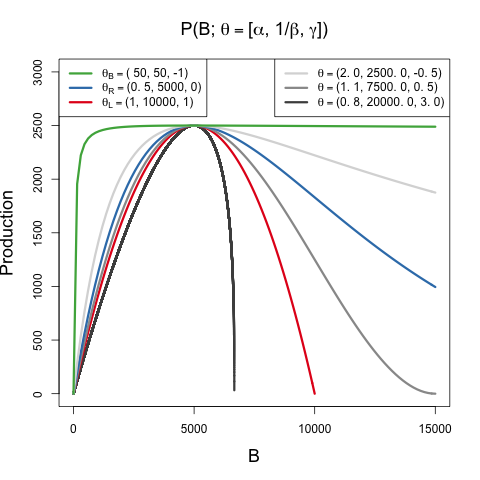
\includegraphics[width=0.5\textwidth]{plots/derisoSrr.png}
%\begin{minipage}[h!]{0.64\textwidth}
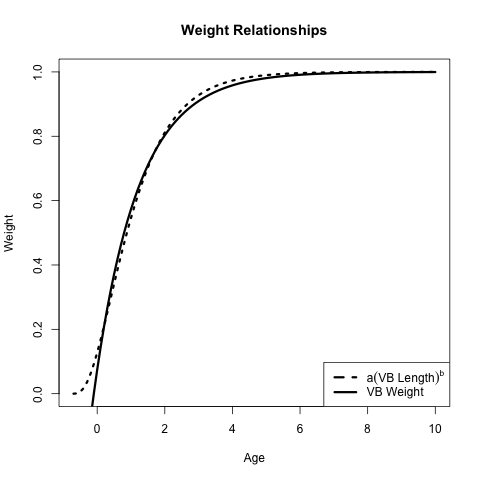
\includegraphics[width=0.49\textwidth]{plots/vbOpt.png}
%\end{minipage}
%\begin{minipage}[h!]{0.3\textwidth}
\vspace{-1cm}
%\hspace*{-1cm}
\caption{
%\onehalfspacing
The typical composition of allometric weight ($b=3$) with VB growth in length, as
approximated by VB growth in weight directly.
%A comparison of 
%with the typical assumption of VB growth in length. 
}
\label{vbComp}
%\end{minipage}
\end{wrapfigure}

%Age structured fisheries models
ASMs typically assume von Bertalanffy %(VB) growth 
\cite[VB]{von_bertalanffy_quantitative_1938} growth in length with age. To model
weight the assumption of VB growth in length, 
$l(a)=l_\infty(1-e^{-\kappa (a-a_0)})$, 
is composed with a power law relating length to weight, $w=al^b$. 
%The statistical model then assumes observed indicies of abundance are proportional to weight. 
%
Since weight is typically proportional to volume, $b$ is usually $\sim3$. When 
$b$ takes a value around $3$ this composition of assumed functional forms %typically 
results in a monotonically increasing sigmoidal curve of weight with 
age. When $b\le1$ weight at age takes a VB-like form with $b=1$ resulting in
an exact correspondence of simultaneous VB-growth in length and weight.

%
The DDM slightly abridges these relationships by directly assuming VB
growth in weight as follows,
%%
%\begin{align}
%\frac{dw}{da} &= \kappa(w_\infty-w(a)) \label{wODE}
%\end{align}
%
\begin{align}
w(a) &= w_\infty(1-e^{-\kappa (a-a_0)}). \label{vbGrowth}
\end{align}
%
Here $\kappa$ is a parameter that controls the instantaneous rate of individual
growth (in weight) with age. $w_\infty$ is the maximum weight of individuals
in the population, and $w(a)$ is the average weight of an individual at
age $a$. The parameter $a_0$ controls the age at which individuals are assumed
to have zero weight; by letting $a_0<0$ this allows fish of age zero to have
positive weight. Rather than taking a sigmoidally increasing function, VB growth
directly in weight results in a monotonically increasing curve that asymptotes
with a strictly decreasing growth rate with age. This results in a curve that
can approximate the composite VB-allometric growth assumption very well except 
at very young ages, see Figure (\ref{vbComp}).
%{\color{red}(only a good approximation for older ages where growth begins to decline)}

%
Together with VB growth, the DDM is derived from the assumption that
both natural mortality and fishing selectivity are both proportional %separately proportional
%the total mortality rate (from both natural and fishing mortality) is proportional 
to a common Heaviside step function with age. That is to say, before a threshold
age of selectivity, $a_s$, no explicit mortality is modeled outside of what is 
implied by the stock-recruitment relationship,
%the population is assumed not to experience anymortality whatsoever, 
but all fish older then $a_s$ experience the same rate
of natural mortality. Simultaneously all fish older than $a_s$ are equally
vulnerable to fishing (i.e. knife edge selectivity at age $a_s$), although
fishing effort may vary through time. Maturity is also assumed to be knife edge at age $a_s$, with only 
mature fish recruiting into the population.

%
Together the parameters $\kappa$ and $a_s$ control individual growth and 
maturity of the stock. Larger values of $\kappa$ represent faster growing 
individuals; in the limiting case where $\kappa\to\infty$ individuals recruit 
at $w_\infty$. Since this DDM ties maturity and selectivity together, $a_s$ can 
also be thought of as controlling the average age of maturity into the reproducing 
stock. Since faster growing stocks tend to mature at younger ages, $\kappa$ 
and $a_s$ tend to be negatively correlated. Furthermore when $\kappa\to\infty$ simultaneously 
with $a_s\to0$, as consistent with the negative correlation between the parameters, 
the DDM converges to the previously studied SPM.

%
Walters \cite{walters_continuous_2020} (preceded with similar discrete time models 
by Deriso \cite{deriso_harvesting_1980} and Schnute \cite{schnute_general_1985}) 
shows that within the above assumptions, the following delay-differential system of 
equations describes %exactly models 
the population dynamics of the total mature, exploitable biomass $B(t)$ and number of individuals $N(t)$ through time.
%%
%\begin{align}
%B(t) = \int^\infty_{a_s} N(a, t)w(a) da
%\end{align}
%
\begin{align}%\kappa->0 slower than a0->\infty
%B(a, t) &= w(a, t)N(a, t)\\ 
%\frac{dB}{dt} &= \overbrace{w(k)R(B(t-k))}^\text{Recruitment Biomass} + \overbrace{\mu w_\infty N(t)}^\text{Growth} - \overbrace{(M+F(t)+\mu)B(t)}^\text{Biomass Loss}\\
&\frac{dB}{dt} = w(a_s)R(B;\theta) + \kappa \left[w_\infty N-B\right] - (M+F)B \label{bEq}\\
&\frac{dN}{dt} = R(B;\theta) - (M+F)N \label{nEq}
%&R(B;[\alpha, \beta, \gamma]) = \alpha B(t-a_s)(1-\beta\gamma B(t-a_s))^{\frac{1}{\gamma}} \label{srr}\\
%&w(a) = w_\infty(1-e^{-\kappa a}) \label{vbGrowth}
\end{align}

%
This formulation separates the number of individuals in the population from the
biomass of the population. The dynamics of $N$, as seen in Eq (\ref{nEq}), are
very similar to that of the production model in Section (\ref{sModel}), 
however the role of the production function is now filled by a ``recruitment''
function, $R(B)$, which describes the number of new individuals recruiting into the
exploitable population as a function of exploitable biomass. In turn, the biomass
dynamics are coupled to the numbers dynamics by the assumption of VB growth with
growth parameters appearing in Eq (\ref{bEq}), converting population numbers
into biomass and accounting for the growth of biomass with age.

%
Eq (\ref{bEq}) of the above model expands the notion of biomass production into the
processes of recruitment, individual growth, and maturity. The term $w(a_s)R(B;\theta)$
represents the biomass of new recruits; with $w(a_s)$ representing the weight of individuals
at the age of maturity/selectivity, $a_s$, and $R(B;\theta)$ representing the number of new recruits
entering the exploitable population at time $t$. The negative term, $(M+F)B$, represents all
causes of mortality as it is applied to biomass. Finally, the term $\kappa \left[w_\infty N-B\right]$
accounts for the net growth of the existing biomass by discounting the limiting maximal individual
growth rate by metabolic weight loss proportional to $B(t)$. 
This structure, as derived from the assumption of simultaneous knife-edge maturity and selectivity, and 
the delay structure in $R$, 
%This term, together with the delay structure in $R$, 
provides the major computational savings of the delay differential setting, as
compared with full ASMs. The mean size and growth associated with changes in recruitment as cohorts 
mature into the population are automatically described by the DDM equations rather than the 
numerous numerical arrays used by ASMs to track quantities across all age classes in time.
% of changes in the mean
%size and growth associated with changes in recruitment as cohorts mature into the population.
%The framework is likely to perform very well at this task, considering that growth and natural 
%survival rates tend to be fairly stable over time in fishes.

%
Often a BH functional form is assumed for the stock recruitment relationship, but many %adequatly flexible 
families of functions may model this relationship. For the sake of evaluating the adequacy
of assumed BH recruitment, the simulation described in the following sections is derived for the 
DDM under the assumption of generalized three-parameter Schnute recruitment,
%
\begin{align}
R(B;[\alpha, \beta, \gamma]') = \alpha B(t-a_s)(1-\beta\gamma B(t-a_s))^{\frac{1}{\gamma}}. \label{srr}
\end{align}
%
The parameters $\bm{\theta}'=[\alpha, \beta, \gamma]$ %\alpha$, $\beta$, and $\gamma$, 
function similarly in this setting as previously described in Section (\ref{sModel}).
That said, since the DDM explicitly parses out growth in its dynamics,
these parameters only describe the net processes of reproduction %larval production %, and maturation into the population, 
where as the production model uses these parameters to also model the net 
effects of growth on biomass production. %NOTE: production model includes net growth in in the nonlinear form of P, while the delay model used VB Growth params (functional form) on top of this nonlinearity. 
The $\gamma$ parameter generalizes the family to model varying degrees of
decreasing recruitment for large biomasses as $\gamma$ increases. The Schnute
function is again exactly equivalent to BH recruitment at the special case when
$\gamma=-1$, it passes through the Ricker model as $\gamma\rightarrow0$, and
Logistic recruitment occurs when $\gamma=1$.

%%the exploitable biomass of the population becomes large
% controls the behavior of recruitment from the special case of BH recruitment at $\gamma=-1$, 
%The structure of the Schnute function here is similar to that of the previously described, with $\gamma$ . 
%
Since the DDM assumes knife edge selectivity, at age $a_s$, the term
$B(t-a_s)$ appears in $R$. That is to say, fish recruiting into the exploitable
population are the result of larval production of biomass $a_s$ time
units in the past. This is because fishing selectivity is only assumed to occur
for fish that are at least $a_s$ time units old and thus fish younger than $a_s$
are not exploitable. This waiting period requires that new recruits be the
result of spawning biomass $a_s$ time units in the past. Modeling maturity and 
selectivity in this way results in dynamics equations which are a system of 
delay differential equations as opposed to the simple ODEs that arise in the 
production model setting.
%which is where the delay differential equation  

%%
%\begin{itemize}
%        %\item parameters $\alpha$, $\beta$, and $\gamma$,
%        %\item The BH and Logistic production functions arise when $\gamma$ is fixed to -1 or 1 respectively. 
%        %\item The Ricker model is a limiting case as $\gamma\rightarrow0$. %\shortcite{schnute_general_1985}.
%        %\item For $\gamma<-1$ a family of strictly increasing Cushing-like curves arise,
%        %       culminating in linear production as $\gamma\to-\infty$. These special cases form
%        %       natural regimes of similarly behaving production functions as seen in Figure (\ref{sRegimes}).
%        %\item time delay
%        \item[$\sim$] interpretation of recruitment (larval production, recruitment) [growth external] vs. production (larval production, recruitment, growth)
%\end{itemize}
%
%\begin{itemize}
%\item general structure: \cite{walters_continuous_2020} \cite[pg. 334]{hilborn_quantitative_1992}
%\item growth: \cite{von_bertalanffy_quantitative_1938}
%\item recruitment: \cite{schnute_general_1985, schnute_analytical_1998}
%\end{itemize}

%
\subsection{Reference Points\label{ddmRP}}

%
Deriving reference points for the DDM under Schnute recruitment is
conceptually similar to the SPM setting. The additional nonlinear
VB growth assumption, alongside Schnute recruitment, quickly makes the
expressions look somewhat unwieldy. Although complicated by growth parameters, 
analytical solutions can still be derived for most of the same quantities as 
was done in Chapter (\ref{schnuteChapter}). 
%(although complicated by growth parameters).

%
Starting from Eqs. (\ref{bEq}) and (\ref{nEq}), setting both $\frac{dB}{dt}$
and $\frac{dN}{dt}$ simultaneously equal to zero, and solving for $B$ and $N$
as a function of fishing, gives the equilibrium biomass and numbers equations.
%
\begin{align}
\bar{B}(F) &= \frac{1}{\beta\gamma} \left( 1 - \Big(\frac{(F + M) (F + M + \kappa)}{\alpha w(a_s)(F + M + \kr)}\Big)^\gamma\right) \label{BF}\\
%\end{align}
%\begin{align}
\bar{N}(F) &= \frac{\alpha\bar{B}(F)(1-\beta\gamma\bar{B}(F))^{1/\gamma}}{F+M} \label{NF}
\end{align}
%
Eq. (\ref{NF}) is just $\frac{R(\bar{B})}{F+M}$, and is coupled to $\bar{B}(F)$
where most of the dynamics appear. Eq. (\ref{BF}) resembles Eq (\ref{BsEq})
from the simple production model setting although the growth parameters
$\kappa$, $w_\infty$ and $w(a_s)$, make slight adjustments to the balance of the
maximum rate of recruitment and mortality rate to give an expression for
equilibrium biomass that accounts for the factors of individual growth.
% for the produce to a more complex expression for equilibirum biomass.

%
Expressions for $B_0$ and $B^*$ are attained by evaluating $\bar{B}(F)$ at
$F=0$ and $F=F^*$ respectively. The calculation of $F^*$ typically involves %amounts to %requires %Obtaining an expression for 
maximization of equilibrium yield, \mbox{$\bar{Y} = F\bar{B}(F)$.} Just as was 
the case under the Schnute SPM in Chapter (\ref{schnuteChapter}), it is again not
possible to analytically maximize $\bar{Y}$ under the Schnute model in the DDM setting. 
However stable numerical solutions for calculating $F^*$ were obtained by 
numerically solving for the roots of the analytical derivative of equilibrium 
yield with respect to $F$. Below a greatly simplified expression for $\frac{d \bar{Y}}{dF}$ 
is shown; the substitution $Z=F+M$ (total mortality rate) has been made to 
produce a more compact expression.
%\vspace{-0.75cm}
\begingroup
\scriptsize
\begin{align}
\frac{d \bar{Y}}{dF} &= \frac{1}{\beta\gamma}\left[ 1 - \one - \two \left( 1 + \thr \right) \right]\label{dBdFS}
%&= (1-\left(\frac{(F+M)*(F+M+\kappa)}{\alpha*(F*w(a_s)+M*w(a_s)+\kappa*w_infty)}\right)^\gamma-(F*(((F+M)*(F+M+\kappa))/(\alpha*(F*w(a_s)+M*w(a_s)+\kappa*w_infty)))^(\gamma-1)*\gamma*(\alpha*(F*w(a_s)+M*w(a_s)+\kappa*w_infty)*(2(F+M)+\kappa)-(F+M)*(F+M+\kappa)*\alpha*w(a_s)))/(\alpha*(F*w(a_s)+M*w(a_s)+k*w_infty))^2)/(\beta\gamma) \label{dBdFS}.
%&= ( 1-\Big(\frac{(F+M)(F+M+\kappa)}{\alpha w(a_s)(F+M+\kappa w_\infty/w(a_s))}\Big)^\gamma - ( F*( ((F+M)*(F+M+\kappa))/(\alpha*(F*w(a_s)+M*w(a_s)+\kappa*w_infty)) )^(\gamma-1)*\gamma*(\alpha*(F*w(a_s)+M*w(a_s)+\kappa*w_infty)*(2(F+M)+\kappa)-(F+M)*(F+M+\kappa)*\alpha*w(a_s)) )/( \alpha*(F*w(a_s)+M*w(a_s)+k*w_infty))^2)/(\beta\gamma) \\
\end{align}
\endgroup
%
$F^*$ is calculated as the numerical root, w.r.t. $F$, of the above expression.
The numerical root is calculated using the base R uniroot function which
employs a derivative free search given by \cite{brent_chapter_1973}. %\shortciteA{brent_chapter_1973}.

%
\subsubsection{BH Constraint}

%
In the SPM the BH constrained RPs are fixed to $\frac{1}{x+2}$, where $x=\frac{F^*}{M}$.
In the DDM the constrained BH RP set is complicated by the growth parameters 
$a_s$ and $\kappa$. Under BH recruitment these parameters slightly %of the DDM slightly %the growth parameters $a_s$ and $\kappa$  
influence this relationship as seen in Figure (\ref{rpSpace}). That said,
the influence of $a_s$ and $\kappa$ on RPs is still largely limited to a
confined region of reference point space which resembles the $\frac{1}{x+2}$
form. In fact the confined region of RPs is bounded above by $\frac{1}{x+2}$. %bounding the region above by $\frac{1}{x+2}$.
In Figure (\ref{rpSpace}) notice that for values of $a_s$ and $\kappa$ that
result in high $w(a_s)$ (high values of $\kappa$ and small values of $a_s$ %seen
%
\begin{wrapfigure}{r}{0.50\textwidth} %[17]{r}[0pt]{0pt}%
%\begin{figure}[h!]
%\vspace{-2.75cm}
%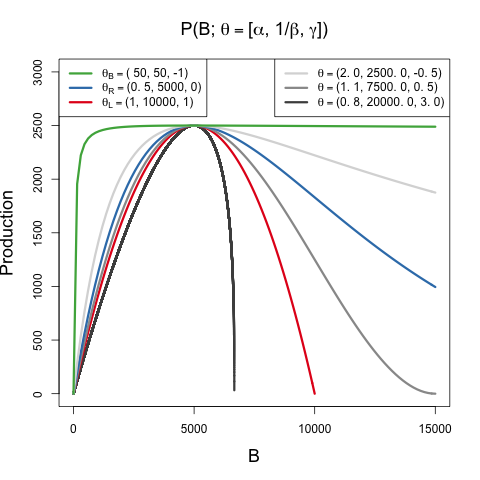
\includegraphics[width=0.5\textwidth]{plots/derisoSrr.png}
%\begin{minipage}[h!]{0.64\textwidth}
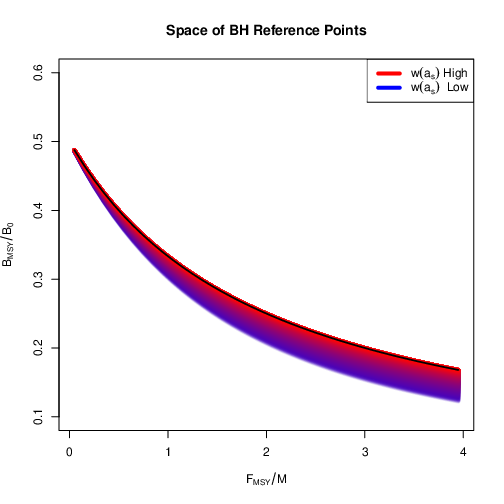
\includegraphics[width=0.54\textwidth]{../ddBias/rpSpaceww.png}
%\end{minipage}
%\begin{minipage}[h!]{0.3\textwidth}
\vspace{-1.5cm}
%\hspace*{-1cm}
\caption{
%\onehalfspacing
The space of BH RPs for the delay model as a function of $\kappa$ and $a_s$.
The RP space is plotted for $80\times80$ combinations of $\kappa\in[0.1, 2]$
and $a_s\in[0.1, 10]$. The color drawn is the resulting value of $w(a_s)$
mapped between blue and red.
%the result of mapping $\kappa$ and $a_s$ values to the red and blue components of the RGB color model repsectively (with G=0). 
$\frac{1}{x+2}$ is plotted in black for reference.
%
}
\label{rpSpace}
%\end{minipage}
\end{wrapfigure}
%\end{figure}
seen in red) the BH RP space converges to $\frac{1}{x+2}$ as derived in the simple
production model setting. Opposing the SPM limit, when $w(a_s)$ is low 
(as seen in the more blue region of Figure(\ref{rpSpace})), RPs decrease as 
the influence of growth in the dynamics increases (i.e. slower individual growth). 
This is another way (this time in RP space) of noticing that the DDM converges 
to the previously studied SPM as $\kappa\to\infty$ and $a_s\to0$ simultaneously.
%When κ → ∞ simultaneously with as → 0, as con-
%1055sistent with the negative correlation between the parameters, the DDM converges to the
%1056previously studied SPM.
%The opposite limit with low values of $\kappa$ and high values $a_s$ (blue region) depresses RPs away from $\frac{1}{x+2}$. 
%{\color{red}emphasize how DDM reverts to SPM}

%
\subsection{Simulation Design\label{delayDesign}}

%
Similarly as previously described in Section (\ref{sSim}) the relationship
between \mbox{RPs $\mapsto$ $\theta$} cannot be fully expressed analytically for the
Schnute DDM. However, just as in the SPM setting, %production model setting,
simulation only requires enough knowledge of these mappings to gather a list
of $(\alpha, \beta, \gamma)$ tuples and the corresponding RPs in some reasonable
space-filling design over RP space. %for the purposes of simulation 

%Like the Schnute production model setting, 
In the DDM a partial mapping for
$\big(F^*, B_0\big) \mapsto \big(\alpha(\cdot, \gamma), ~\beta(\cdot, \cdot, \gamma)\big)$
%in the delay modelling setting 
can be derived analytically in terms of RPs and $\gamma$. The substitution
$Z^*=F^*+M$ is made where $F^*$ and $M$ appear together to produce a more
compact expression.

%
\begingroup
\scriptsize
\begin{align}
\alpha & = \left[ \oneA + \twoA \left( 1 + \thrA \right) \right]^{\frac{1}{\gamma}} \label{aDelay}\\
\beta &= \frac{1}{\gamma B_0} \left( 1 - \Big(\frac{M (M + \kappa)}{\alpha w(a_s)(M + \kr)}\Big)^\gamma\right) \label{bDelay}%\\
%\frac{B^*}{B_0} &= \frac{ 1 - \Big(\frac{(F^* + M) (F^* + M + \kappa)}{\alpha w(a_s)(F^* + M + \kr)}\Big)^\gamma }{ 1 - \Big(\frac{M (M + \kappa)}{\alpha w(a_s)(M + \kr)}\Big)^\gamma }
\end{align}
\endgroup

%
Above Eq. (\ref{aDelay}) results from setting \mbox{Eq. (\ref{dBdFS})} equal to zero
and solving for $\alpha$, and \mbox{Eq. (\ref{bDelay})} results from solving the
$\bar{B}(0)$ expression, as derived from \mbox{Eq. (\ref{BF}),} for $\beta$. The system
is completed by further working with the $\frac{\bar{B}(F^*)}{\bar{B}(0)}$ expression,
as seen below, to identify $\gamma$.
\begin{align}
\frac{B^*}{B_0} &= \frac{ 1 - \Big(\frac{(F^* + M) (F^* + M + \kappa)}{\alpha w(a_s)(F^* + M + \kr)}\Big)^\gamma }{ 1 - \Big(\frac{M (M + \kappa)}{\alpha w(a_s)(M + \kr)}\Big)^\gamma }
\label{gDelay}
\end{align}

%
The system formed by collecting Eqs. (\ref{aDelay}), (\ref{bDelay}), and 
(\ref{gDelay}) can be navigated similarly to Eq. (\ref{abgSys}) in the Schnute 
production model setting. For a population experiencing natural mortality $M$, 
VB growth with parameters $\kappa$ and $w_\infty$, and age of selectivity $a_s$ 
the above system can fully specify $\alpha$ and $\beta$ for a given $\gamma$, 
by fixing $F^*$, $B_0$, and $\frac{B^*}{B_0}$. For a given $\gamma$ a cascade 
of closed form solutions for $\alpha$ and $\beta$ can be obtained, just as in 
Section (\ref{sSim}). 
%
First $\alpha(\gamma)$ can be computed, and then $\beta(\alpha(\gamma), \gamma)$ 
can be computed. If $\alpha(\gamma)$ is filled back into the expression for 
$\frac{B^*}{B_0}$, the system collapses into a single onerous expression for 
$\frac{B^*}{B_0}(\alpha(\gamma), \gamma)$. For brevity, define the function 
\mbox{$\zeta(\gamma)=\frac{B^*}{B_0}\big(\alpha(\gamma), \gamma, F^*, M\big)$} 
based on Eq. (\ref{gDelay}).

%
Again rather than inverting $\zeta(\gamma)$ for $\gamma$, $\gamma$ is the
sampled so that the overall simulation design is space filling as described in
Section (\ref{sLHS}). Given the sampled $\gamma$, the cascade of $\alpha(\gamma)$, 
and then $\beta(\alpha(\gamma), \gamma)$, can be computed, and the Schnute DDM 
is fully defined by a given $(\frac{F^*}{M}, \frac{B^*}{B_0})$.
%
While conceptually this framing is similar to the Schnute SPM,
the analytical expressions are more complex, and numerically treacherous, since
growth parameters appear explicitly here. Other ways of navigating the RPs $\mapsto$ $\theta$
system are possible, but for the sake of numerical stability this strategy has
proven the most reliably accurate by limiting exposure to numerical error 
propagation which quickly becomes significant using other schemes.

%
Each design location defines a complete Schnute DDM with
the given RP values. Just as in Chapter (\ref{schnuteChapter}), $B_0$ is fixed 
at $10000$, $q$ is fixed at $0.0005$, and $M$ is fixed at $0.2$; furthermore $a_0$ and $w_\infty$ (of VB 
growth) were fixed to -1 and 1 respectively throughout.
The values of $\kappa$ and $a_s$ are varied roughly along the line $w(a_s)=w_\infty-\frac{a_s}{3}$ 
so as to produces a negatively correlated relationship between $\kappa$ and 
$a_s$ representing fast ($\kappa=10$,  $a_s=0.1$), medium ($\kappa=0.5$,  $a_s=1$) and 
slow ($\kappa=0.1$,  $a_s=2$) individual growth simulation settings.
Indices of abundance are simulated from the Schnute model at each design 
location, a small amount of residual variation, $\sigma = 0.01$,
is added to the simulated index, and the data are then fit with a misspecified
BH model. $\sigma$ is later relaxed to $0.12$ in Section (\ref{oscillation}). The design captures various degrees of model misspecification
relative to the BH model, so as to observe the effect of recruitment
misspecification upon RP inference.

%{\color{red} hint at larger $\sigma$}

%%
%{\color{red}
%point to catch, and LHS design, and Metamodel.
%}
%
%\begin{itemize}
%%$\bm{\phi}$ fixed, $q$ fixed,\\ 
%%MLE $\bm{\theta}$ and $\sigma^2$\\
%%\item fixed $B_0=10000$, $M=0.2$, $a_0=-1$, $w_\infty=1$
%\item play with $\kappa$ and age of selectivity $a_s$
%%Look at values above and adapt from schnute paper.
%\end{itemize}

%
\subsection{Metamodeling}

%
The GP metamodeling method previously developed in Section (\ref{gpmm}), and later adapted 
\mbox{%adapted 
for analysis of the BH model in Chapter (\ref{schnuteChapter}), 
is also used in the DDM setting here.
}
%and (\ref{delayChapter}) for the
%analysis of BH RP inference with the following modifications.

%%
%Recall that each design location of the simulation uniquely represents a three parameter
%Schnute model. Index of abundance data are generated from the Schnute model
%at each design location to be fit with a two parameter BH model.
%The productivity parameters of the estimated BH model are reparameterized as
%$\log(\alpha)$ and $\log(\beta)$ so that the modeled spaces are each in $\mathbb{R}$.
%In turn, the MLE and associated variance (via the inverted Fisher information)
%of these reparameterized quantities propagate the vectors
%$\textbf{y}$ and $\bm{\omega}$ respectively to be modeled by the GP metamodel.
%These quantities along with the RP calculations derived in each respective chapter
%fully specifies the metamodeling analysis with all other details remaining the same.
%%be a vector of estimates of the estimator variances (via the
%%inverted Fisher information) at each $\textbf{y}$.
%\

%%
%{\color{red}
%point to catch, and LHS design, and Metamodel.
%}

%%
%\subsection{Clustering Model Failure}
%
%%
%Considering the behavior observed in Section (\ref{schnuteLowResults}), where
%$\frac{F^*}{M}$ is dramatically underestimated, it is natural to ask
%where specifically in RP space we might see this catastrophic failure of the
%BH model as growth assumptions change.
%%
%%The structure of RPs under the BH model suggests several potential avenues for
%%forming hypotheses to identify highly misspecified RP regions. 
%%however identifing cases where $\frac{F^*}{M}$
%%but the single
%%clearest feature to identify are cases where $\frac{F^*}{M}$ is
%%heavily under-estimated. 
%%Here a hypothesis testing inspired framework is used to identify these cases.
%%By using the GP metamodel to propagate estimate uncertainty across the simulated 
%%RP space the metamodel can predict which stocks may fail when modeled under 
%%the BH model. 
%Below a hypothesis testing inspired classifier is derived in terms of the GP predictive structures 
%for identifying where BH inference fails in this way. 
%%% of misspecified BH RPs.
%%%as a surrogate for the distribution of 
%%%$\frac{F_{MSY}}{M}$ across degrees of misspecified BH models. 
%%This allows for a rejection threshold (against the null hypothesis that BH RP
%%estimates are unbiased) to be derived in terms of the GP predictive structures
%%to define a classifier for identifying where BH inference breaks down
%%broadly over RP space.
%
%
%%\clearpage
%%
%Recall that the metamodel models MLEs of $log(F^*)$ under the misspecified BH model.
%%is a metamodeled quantity, 
%%corresponding to $$, $log(F_{MSY})$, corresponding to is the metamodeled 
%Thus, for a given set of RPs, $\textbf{x}$, the BH metamodeled
%quantity is given by kriging prediction as $N(\hat y(\textbf{x}), \hat \sigma^2(\textbf{x}))$,
%where $\hat y(\textbf{x})$ is the kriging mean (as previously described in
%Eq. (\ref{gpYHat})) and $\hat \sigma^2(\textbf{x})$ provides estimate
%uncertainty via the kriging predictive variance given by,
%\begin{equation} %k(x) a n−vector with kν,j (x) = K(x, xj ), for all xj ∈ X
%       \hat \sigma^2(\textbf{x}) = \textbf{R(x, x)} - \textbf{r(x)}'\bm{R}^{-1}_{\bm{\ell}}\textbf{r(x)}.
%\end{equation}
%
%%
%Model failure with respect to estimating $\frac{F^*}{M}$ under the BH
%model is measured by the percent error as previously described in Section (\ref{highConRes}).
%When the BH model estimates $\frac{F^*}{M}$ well the percent error is
%expected to be small in the following sense,
%%In this setting to define the degree of model failure the percent error of the 
%%estimate is capped at no more than $P$ 
%%with respect to $\frac{F_{MSY}}{M}$ 
%%the percent error is capped to 
%
%%
%\begin{equation}
%\frac{\frac{F^*}{M}-\frac{\hat{F}^*}{M}}{\frac{F^*}{M}}\le P. \label{pError}
%\end{equation}
%
%%
%$P$ defines the extent of model failure on the scale of percent error. For
%measuring catastrophic model failure $P$ was chosen to be $0.5$, but smaller values
%of $P$ may be chosen to emphasize regions of more subtle model failure. %subtle regions 
%%
%Since $\frac{F^*}{M}$ is generally underestimated for stocks above the BH set, a 
%one-sided test is used to identify model failure.
%Thus, when the percent error is statistically greater than $P$ the notion that
%the BH model estimates $\frac{F^*}{M}$ well (in the sense defined by $P$) is rejected.
%
%%
%For statistical evaluation, it is convenient to rearrange Eq. (\ref{pError})
%as \mbox{$\hat{F}^*\ge (1-P)F^*$}. $\hat{F}^*$ is then distributed as $LN(\hat y(\textbf{x}), \hat \sigma^2(\textbf{x}))$,
%and the rejection region is then defined as the RPs for which the $5^{th}$ percentile
%from the Log-normal distribution falls below \mbox{$(1-P)F^*$.}

%
\subsection{Delay Differential Integration}

%
The delay model belongs to a class of differential equations known as delay
differential equations (DDE). The delay arises from the $B(t-a_s)$ terms
found in the recruitment function. Solving DDEs require special care which
depends on the nature of the time delay. The addition of time-varying delays,
many different delays, or very small delays (delays below the step size of the
numerical integrator) results in some of the more challenging settings for
solving DDEs. However with a single stationary model of the age of selectivity and maturity,
the DDM used here represents one of the most straightforward numerical 
DDE settings. The most numerically challenging case presented here arises
in the case of the limiting SPM when $a_s\to0$ while $\kappa\to\infty$.
That said the limiting SPM can be approximated for values of
$a_s\approx0.1$, and it was straightforward to ensure that the step size of
the integrator remained reasonably below 0.1.

%
The DDE presented here is integrated with the initial values fixed at $B_0$
and $N_0$ as given by Eqs. (\ref{BF}) and (\ref{NF}) with $F=0$ at any given
configuration of $\bm{\theta}$ and growth parameters. %$\kappa$, $w_\infty$ and $a_s$. 
The system given in Eqs. (\ref{bEq}) and (\ref{nEq}) are then solved
numerically using the implicit Livermore Solver (lsode) as implemented in the
\verb|dede| function of the R package \verb|deSolve| \cite{soetaert_solving_2010}.
The \verb|dede| solver provides many methods for integrating DDEs, but lsode
was chosen because it is an implicit method that runs relatively quickly with
a relatively smaller footprint in system memory as compared with other methods.
The radau method was also tried in more computationally challenging settings
with good results (albeit running more slowly that lsode). Ultimately the
simulated parameter space did not produce DDEs that require the more expensive
radau integrator to solve accurately.

%delays are on the order of the step size (vanishing delays) are difficult to solve. (dde CRAN)
%
%https://cran.r-project.org/web/packages/dde/vignettes/dde.html

%
\subsection{Parameter Estimation}
%%
%\begin{itemize}
%        %\item layout likelihood setup
%        %\item mention recreational data numbers likelihood
%        %\item point out similarity of B/N solutions
%        \item I use B only here
%        \item quick statement of inference, and reference to previous section
%\end{itemize}

%
Let $I_t$, $t\in\{1,2,3,...,T\}$, be a series of indices of abundance, 
proportional to biomass, as simulated from the Schnute DDM. These data 
are modeled with the following log-normal observation model that has been 
intentionally constrained to BH recruitment, 
%is then intentially constrainted to BH recruitment and a log-normal observation model as follows, % by fixing $\gamma=-1$.
%Growth parameters: $\bm{\phi}'=[\kappa, w_\infty, a_0, a_s]$
%
%The observation model for the fitted model is log-normal such that, 
%|q, \sigma^2, \bm{\theta}, \bm{\phi}
\begin{align}
I_t \sim LN(q B_t(\bm{\theta}, \bm{\phi}), \sigma^2). \label{bL}
\end{align}
%
$B_t(\bm{\theta}, \bm{\phi})$ is the biomass solution of the BH constrained DDE system. %of DDE defined in Eq. (\ref{bEq}). 
The BH constraint is implemented by fixing $\gamma=-1$ so that $\bm{\theta}'=[\alpha, \beta, \gamma=-1]$. 
$\bm{\phi}$ is a vector of growth and maturity parameters, 
$\bm{\phi}'=[\kappa, w_\infty, a_0, a_s]$. The nuisance parameter $q$ models 
the proportionality constant of the index with process biomass, and $\sigma^2$ 
models residual variation of the index.

%
In this setting, $\bm{\phi}$ is fixed %and $q$ are fixed %at the true value of 0.0005 
to focus on the inferential effects of model misspecification on recruitment
parameters and RPs. Typically $\bm{\phi}$ is not well informed by index data and %Under the BH model  and typically
would be estimated externally to the DDM for data-limited stocks.
%
%Without an explicit mechanism for the DDM to incorporate
%age data, under the BH model $\bm{\phi}$ is not well informed and would
%tyically be estimated externally for data limted stocks. 
%%
%Under BH recruitment $\phi$ can only have a modest impact the range of modeled RPs, 
%when compared with $\theta$, as demonstrated in Figure (\ref{rpSpace}).
%%
%the BH model only contributes largly unimportant for the mapping of RPs since  
%{\color{red} $\bm{\phi}$ tyically estimated externally; 
%the components of $\phi$ only slightly impact RPs as seen in Figure (\ref{rpSpace})}.

%
$\sigma^2$ and $\theta$ are reparameterized to the log scale and fit via MLE.
Transforming the parameters to the log scale improves the reliability of
optimization, in addition to facilitating the use of Hessian information for
estimating MLE standard errors. Given that the biological parameters enter the
likelihood via a nonlinear differential equation, and further the parameters
themselves are related to each other nonlinearly, the likelihood function can
often be difficult to optimize. A hybrid optimization scheme is used to
maximize the log likelihood to ensure that a global MLE solution is found. The
R package GA \cite{scrucca_ga_2013, scrucca_extensions_2017} is used to
run a genetic algorithm to explore parameter space globally. Optimization
periodically jumps into the L-BFGS-B local optimizer to refine optima within a
local mode. The scheme functions by searching globally, with the genetic
algorithm, across many initial values for starting the local gradient-based
optimizer. The genetic algorithm serves to iteratively improve hot starts for
the local gradient-based optimizer. Additionally, optimization is only
considered to be converged when the optimum results in an invertible Hessian at
the found MLE.

%
\subsubsection{Numbers Indices}

%
While not utilized here, ASMs may model %age structured models may model
%the delay model is also capable of modeling 
indices as proportional to numbers rather than (or simultaneously to)
biomass. When solving the DDE, Eq. (\ref{nEq}) points out that the full DDE
solution will expose a numbers solution simultaneously with a biomass solution
that may be used for these purposes. These solutions are often quite similar
since the main driver of process behavior comes from the form of $R$ which is
shared among $N$ and $B$.
However, it is common on the west coast of the US that indices derived from commercial
fisheries are measured as weights %biomass Index observations
while indices derived from recreational fisheries are often measured as counts.
%represent indicies that are better modeled as proportional tocounts rather than biomass. 
If a numbers index, $J_t$, is observed alongside the previously
mentioned biomass index, the following likelihood component can be added as a %is often added as a
conditionally independent component of the likelihood, %as follows,
%|p, \tau^{2}, \bm{\theta}, \bm{\phi}
\begin{align}
J_t \sim LN(p N_t(\bm{\theta}, \bm{\phi}), \tau^{2}) \label{nL}.
\end{align}
%
$N_t(\bm{\theta}, \bm{\phi})$ is the numbers solution of the DDE system.
$\bm{\theta}$ and $\bm{\phi}$ are the productivity and growth parameters shared in 
common with the biomass component. $p$ and $\tau^2$ are then the analogous
proportionality constant and residual variation of the numbers index respectively.

%
\clearpage
There may be many other useful ways to build observation models from the 
numbers and biomass DDE solutions. For example, one may develop 
models around the quantity $\frac{B(t)}{N(t)}$ to model the average size of 
individuals in the population through time. By including average size data, 
with stationary models of mortality, this model may resolve uncertainty around 
%impied values of 
latent recruitment in time. 
% around around such a likelihood component 
That said, for the purposes of the simulations run here the observation model 
is expressed only in terms of biomass as stated in Eq. (\ref{bL}) of the previous section.
%indicies proportional to biomass are the only  only simulated data is only included only the biomass 

%
%

%\clearpage
\section{Results}

%{\color{red} Biological Regeim corr($a_s$, $\kappa$)<0}

%Together the parameters κ and as control individual growth and maturity of the
%stock. Larger values of κ represent faster growing individuals; in the limiting case
%where κ → ∞ individuals recruit at w∞ . Since this DDM ties maturity and selectivity
%together as can also be thought of as controlling the average age of maturity into the
%reproducing stock. Since faster growing stocks tend to mature at younger ages, κ and
%as tend to be negatively correlated. When κ → ∞ simultaneously with as → 0, as con-
%sistent with the negative correlation between the parameters, the DDM converges to the
%previously studied SPM.

%The values of κ and
%as are varied roughly along the line w(as ) = w∞ − a3s so as to produces a negatively
%correlated relationship between κ and as representing fast (κ = 10, as = 0.1), medium
%(κ = 0.5, as = 1) and slow (κ = 0.1, as = 2) individual growth simulation settings.

%\begin{figure}[h!]
\begin{wrapfigure}{r}{0.50\textwidth}
\vspace{-1.5cm}
%\vspace{-0.5cm}
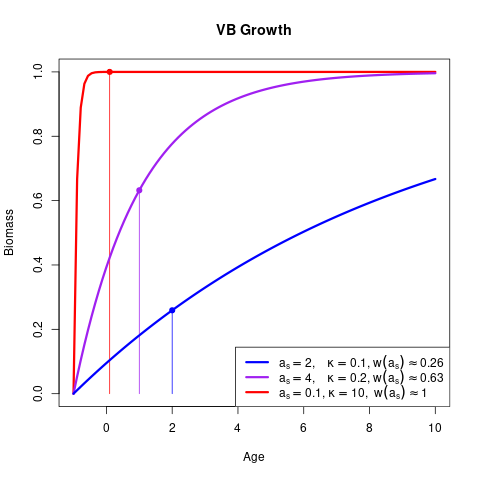
\includegraphics[width=0.49\textwidth]{../ddBias/vbCurves.png}
%\vspace{-1cm}
\caption{Three hypothetical individual-growth curves, demonstrating 
fast (i.e. SPM limit), medium and slow individual growth in red, 
purple, and blue respectively.
\label{vbCurves}}
\end{wrapfigure}
%
Figure (\ref{vbCurves}) shows the VB growth curves in weight
described at the end of Section (\ref{delayDesign}). %spanning a range of individual growth and maturity parameters and a range of RPs. 
The larger values of $w(a_s)$ correspond to larger recruits relative 
to maximum size; by comparing the RPs of models with larger values of 
$w(a_s)$ in Figure (\ref{rpTriptic}) we can see that these models result in SPM-like RPs.
When $w(a_s)$ is large, recruits are near maximum size and thus there is little growth left 
% to be This leaves little growth 
to be evaluated by the biomass dynamics equations. In Figure (\ref{vbCurves}) the red curve 
demonstrates a stock with fast growing individuals that provides an example of the SPM limit 
($a_s\rightarrow0$ and $\kappa\rightarrow\infty$). In this setting individuals recruit so near maximum size that 
growth does not meaningfully effect the biomass dynamics in this setting \mbox{(i.e. $w(a_s)\approx w(a_s+1)\approx w(a_s+2)...$).}
%with no growth in the dynamics(no growth) production model limit ($a_s\rightarrow0$ and $\kappa\rightarrow\infty$).
The cases shown with smaller $w(a_s)$ values (the purple and blue curves) correspond to 
incrementally slower growth behaviors. The slowest growth stock simulated is the blue curve, 
where $a_s=2$ and $\kappa=0.1$, emphasizing the effect of growth on the biomass dynamics. 
% most amoung these examples. 
%representing the most\dramatic growth shown here.
%a more lagged selectivity and slow indivdual-growth.

%
\begin{figure}[h!]
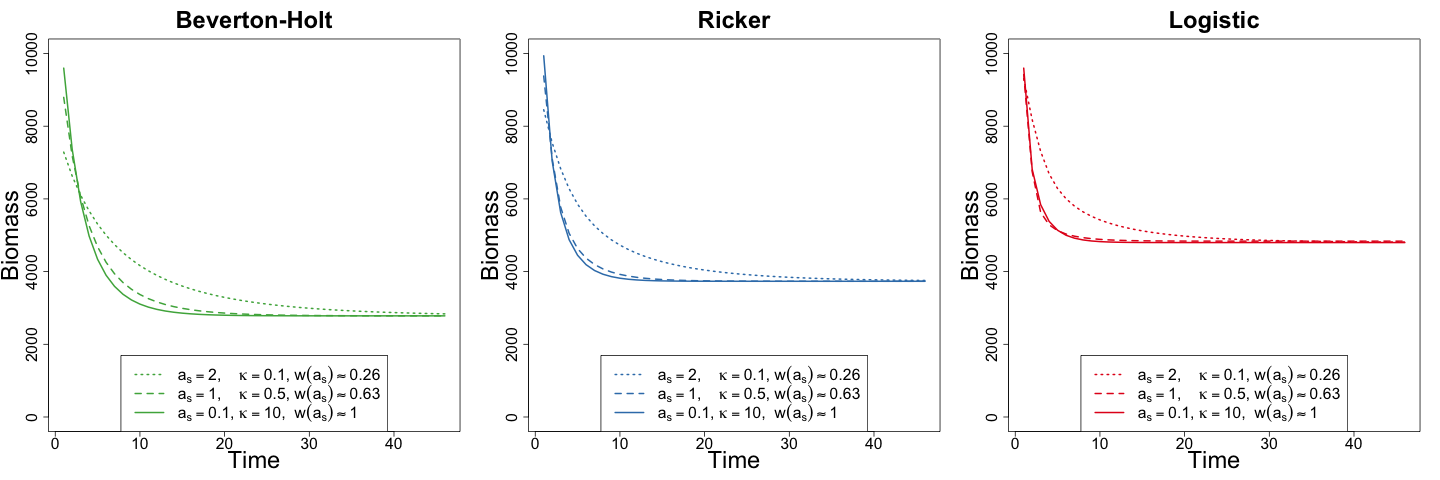
\includegraphics[width=\textwidth]{../ddBias/growthTriptic.png}
\vspace{-0.5cm}
\caption{
Biomass dynamics of BH ($left$), Ricker ($center$), and Logistic ($right$)
DDMs in the low contrast simulation setting. In all cases
$\alpha=1.2$ and $\beta$ is chosen so that each model shares the same
$B^*$ within each given $\gamma$.
}\label{delayTriptic}
\end{figure}
%
Figure (\ref{delayTriptic}) demonstrates a range of biomass dynamics that the Schnute
DDM can display under this spectrum of growth behaviors with fishing held consistent
at $F^*$. The three special cases of $\gamma=-1$ (BH), $\gamma\to0$
(Ricker), and $\gamma=1$ (Logistic) recruitment are shown in each of the above growth configurations.
%of growth ranging from the simple (no growth) production model setting when 
%$a_s\rightarrow0$ and $\kappa\rightarrow\infty$, to an opposing case ($a_s=10$ 
%and $\kappa=0.1$) representing extremely lagged selectivity and slow indivdual-growth. 
%By reference with Figure (\ref{rpSpace}), notice that the latter individual-growth/maturity 
%configuration represents a RP set in the deep blue regiem, thus 
%this case represents 
%dynamics where RPs are heavily influenced by individual-growth/maturity, 
%rather than solely determined by the assumed functional form of recruitment as is 

 
%%the case with the simple production model. The case $a_s=2$ and $\kappa=0.1$ is 
%%shown as an example of dynamics where RPs are more moderatly influenced by 
%%individual-growth/maturity. 
%%The shortened selectivity lag allows oscillatory individual-growth/maturity 
%%dynamics to quickly equilibrate towards a more purely 
%%recruitment driven dynamics more quickly than the $a_s=10$ example.
%%% right leaning yeild curve
%Notice under the most emphatic growth ($a_s=2$ and $\kappa=0.1$) setting, biomass
%of the Logistic model comes into equilibrium at $B_{MSY}$ as an oscillating
%curve. This effect occures here due to the Logistic model's relatively high $\frac{B^*}{B_0}$
%%steep yeild curve for high biomasses 
%interacting with the lag in selectivity upon the sudden onset of fishing; this
%produces a shock that pushes biomass past $B_{MSY}$ setting up an oscillatory
%pattern of recruitment.
%%over the steepest regions of the yeild curve. 
%One may also observe these oscillations under the Ricker model by exaggerating
%the $a_s$ lag as well as the steepness of the Ricker curve. The BH model may
%also demonstrate these oscillations, in a heavily lagged setting, by shocking
%the population past its relatively low $B_{MSY}$ as a sudden release in fishing applied to a
%%over the steepest portion of its yeild curve (a sudden release 
%heavily fished population at low equilibrium biomass.

%
\begin{wrapfigure}{r}{0.50\textwidth}
\vspace{-0.5cm}
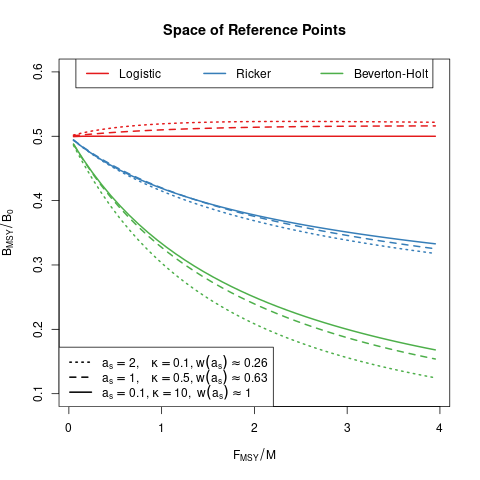
\includegraphics[width=0.49\textwidth]{../ddBias/rpTriptic.png}
\vspace{-0.75cm}
\caption{Restricted RP-space under each recruitment models,
%The dotted lines show the RP-space of each recruitment model
with each growth curve.}\label{rpTriptic}
\end{wrapfigure}
%
Figure (\ref{rpTriptic}) shows the range of RPs that can be modeled with each
of the BH, Ricker, and Logistic recruitments over the spectrum of
individual-growth/maturity models simulated here. Notice for smaller values of 
$\frac{w(a_s)}{W_\infty}$ the further the RP curve lies from the SPM,
and each recruitment model reacts slightly differently under each of the given growth
parameters. The Ricker and BH RP-spaces are qualitatively similar in shape
with smaller values of $w(a_s)$ decreasing $\frac{B^*}{B_0}$ relative to the SPM. 
The Logistic model on the other hand increases $\frac{B^*}{B_0}$ relative to 
the SPM as $w(a_s)$ decreases. It is also worth noting that the Ricker model's
RPs are much less influenced by growth parameters as compared with that of the
BH or Logistic model.

%\clearpage
%
\subsection{Fast Individual Growth (SPM Limit)\label{fast}}

%
Under the delay differential's limiting SPM ($a_s=0.1$ and $\kappa=10$),
the expectation is that RP inference should be identical to that of the model seen in
Chapter (\ref{schnuteChapter}). By way of verifying this equivalence, Figure (\ref{prodLimit})
demonstrates a virtually identical pattern of RP biases as previously seen in
Figures (\ref{contrastTrio}) and (\ref{bhLowArrows}) (under both of the high and
low contrast settings).

%
\begin{figure}[h!]
\begin{minipage}[h!]{0.44\textwidth}
%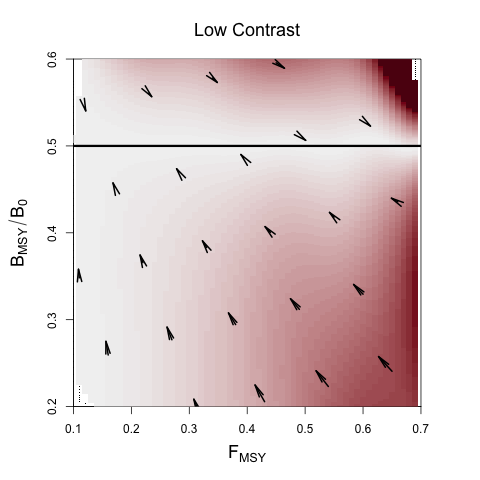
\includegraphics[width=\textwidth]{../ptNew/directionalBiasSubPTFlatT30.png}
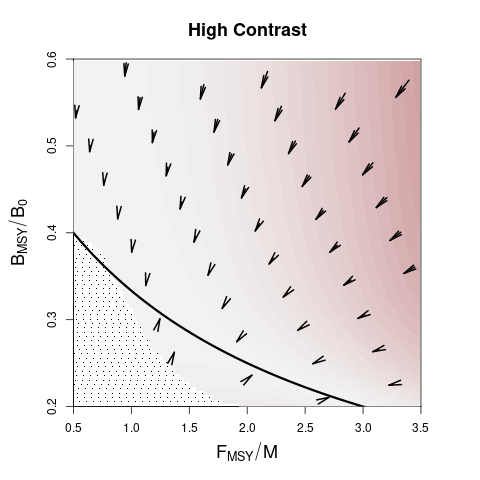
\includegraphics[width=\textwidth]{../ddBias/directionalBiasDDSubExpT45N300AS0.1K10Reds 2.png}
\end{minipage}
\begin{minipage}[h!]{0.44\textwidth}
%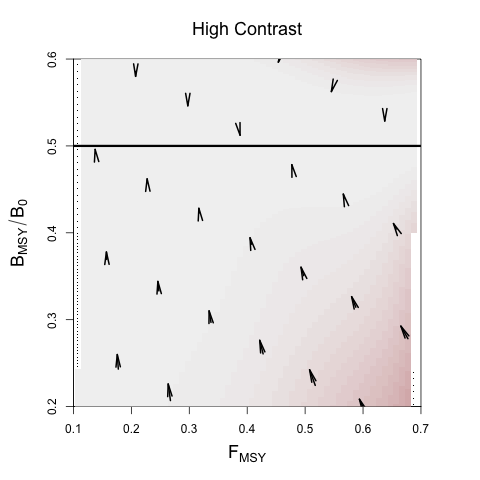
\includegraphics[width=\textwidth]{../ptNew/directionalBiasSubPTExpT45MinCon.png}
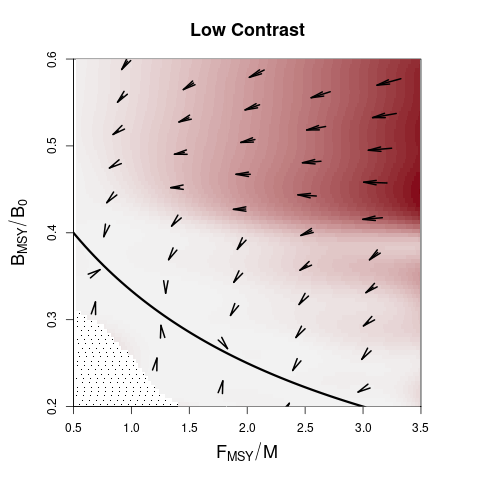
\includegraphics[width=\textwidth]{../ddBias/directionalBiasDDSubFlatT45N150A0-1AS0.1K10N56Reds 2.png}
%directionalBiasDDSubFlatT45N150A0-1AS0.1K10N56.png}
\end{minipage}
\begin{minipage}[h!]{0.09\textwidth}
\hspace{-1cm}
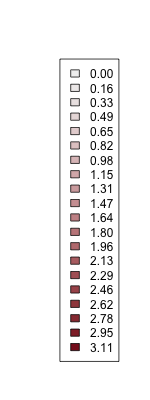
\includegraphics[width=1.5\textwidth]{../gpBias/legendSubSchnute.png}
\end{minipage}
%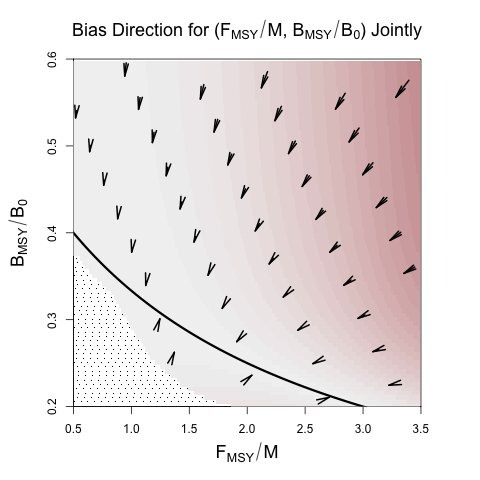
\includegraphics[width=0.49\textwidth]{../ddBias/directionalBiasDDSubExpT45N300AS0.1K10.png}
%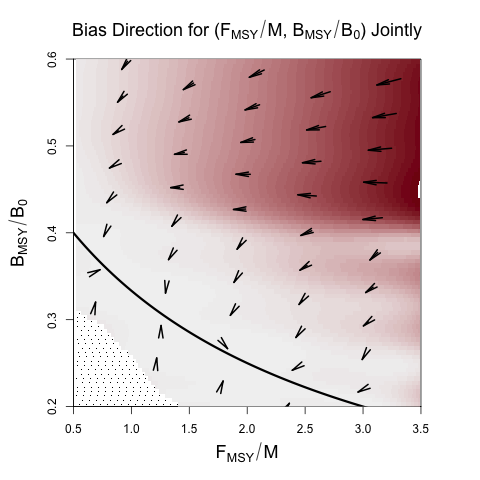
\includegraphics[width=0.49\textwidth]{../ddBias/directionalBiasDDSubFlatT45N150A0-1AS0.1K10N56.png}
\caption{
RP mapping of BH DDM fit to Schnute DDM data under the fast individual growth setting (SPM limit)
%simple (nogrowth) production model limit. 
$(left)$ High contrast simulation.
$(right)$ Low contrast simulation.
}\label{prodLimit}
\end{figure}

%\subsubsection{high}
%Just as seen in Section (\label{schnutePics}), here 
%As a limiting case of the delay model in this case, Figure (\ref{prodLimit}) again demonstrates 
%%Just as seen in Chapter (\ref{schnuteChapter}), Figure (\ref{prodLimit}, $left$)
%how RP mapping

%Again under
Indeed in the high contrast setting, Figure (\ref{prodLimit}, $left$) shows
how the BH model induces the same pattern of bias as seen in Chapter
(\ref{schnuteChapter}). There is bias in both RPs (in accordance with the
$\frac{B^*}{\bar B(0)}=\frac{1}{F^*/M+2}$ RP-set) so as to produce a nearly
minimal distance mapping of RPs onto the constrained BH set of RPs.
%\subsubsection{low}
Similarly, in the low contrast setting, Figure (\ref{prodLimit}, $right$) again
shows the same two regime pattern of RP inference. Firstly, there is a region of
relatively small model misspecification where a similar nearly minimal distance mapping
is preserved. Secondly, as model misspecification becomes greater (around the
Ricker set) $\frac{F^*}{M}$ begins to be sharply underestimated. Above this
break point in RP estimation inference appears to be driven toward the trivial RP
$\frac{F^*}{M}=0$, $\frac{B^*}{\bar B(0)}=0.5$) that is shared in common
among all of the two-parameter models described here.

%
These results confirm that the expected theoretical limiting dynamics do indeed behave 
nearly identical to RP inference patterns previously described. Given the implementation 
differences between the DDM and the SPM this result also provides replicability %some sense of  
of the results in Chapter (\ref{schnuteChapter}). 
%expected RP inference patterns as previously observed in 
%Chapter (\ref{schnuteChapter}).

%
%\clearpage
\subsection{Moderate Individual Growth\label{medium}}

%
Moving past the SPM, other values of $a_s$ and $\kappa$ provide a probe into 
the effects individual growth dynamics may have on RP inference.
%
Individual growth is a multifaceted phenomena that is not easily reduced
to a single number, but for the purposes here $w(a_s)$ serves as a decent 
proxy for the extent of the model dynamics that are due to individual growth. % displayed by the model. 
%
This follows from the intuition that individuals maturing at a smaller fraction
of $w_\infty$ demonstrate the dynamics of growth during an observable (to the model) %being fished (observable) 
phase rather than growth occurring prior to selection. % by the fishery.

%
That said, $w(a_s)$ is not a one-to-one map of $\kappa$ and $a_s$.
%
A level curve of $w(a_s; \kappa)=c$ is attained by increasing the value of $a_s$
and decreasing $\kappa$ correspondingly, or vice versa.
%
The case where $a_s=1$ and $\kappa=0.5$ (resulting in $w(a_s)\approx0.6$)
represents a reasonable example of moderate individual growth.
%biological example of moderate individual growth.
%
Similar examples of the $w(a_s)=0.6$ level curve result in much larger lags
(discussed in Section (\ref{oscillation})) or larger $\kappa$'s which quickly
tend toward behaviors previously described in the SPM setting.

%
\begin{figure}[h!]
\begin{minipage}[h!]{0.44\textwidth}
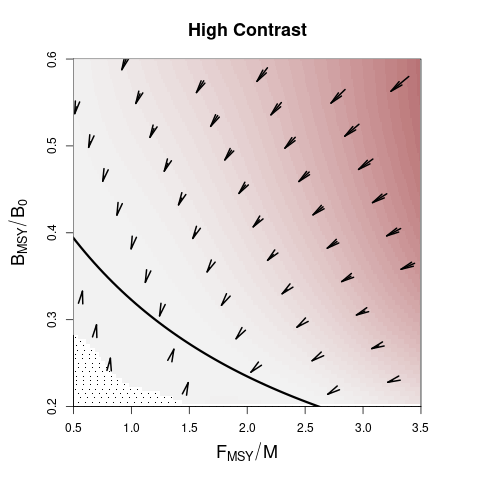
\includegraphics[width=\textwidth]{../ddBias/directionalBiasDDSubExpT45N150A0-1AS4K0.2N38Reds 2.png}
\end{minipage}
\begin{minipage}[h!]{0.44\textwidth}%NOTE: arrow spacing
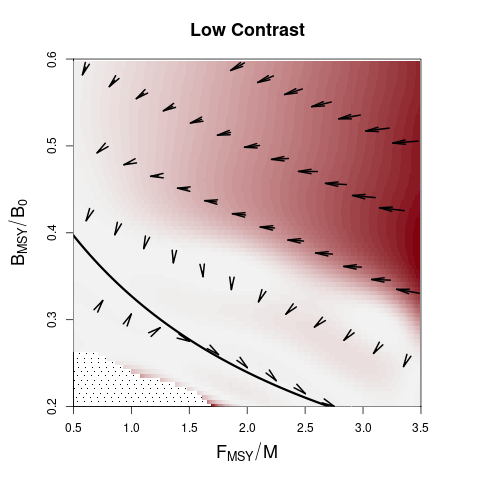
\includegraphics[width=\textwidth]{../ddBias/directionalBiasDDSubFlatT45N150A0-1AS1K0.5N56Reds 2.png}
\end{minipage}
\begin{minipage}[h!]{0.09\textwidth}
\hspace{-1cm}
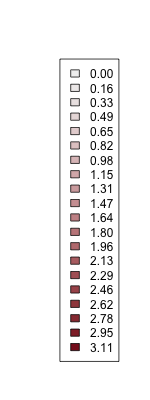
\includegraphics[width=1.5\textwidth]{../gpBias/legendSubSchnute.png}
\end{minipage}
%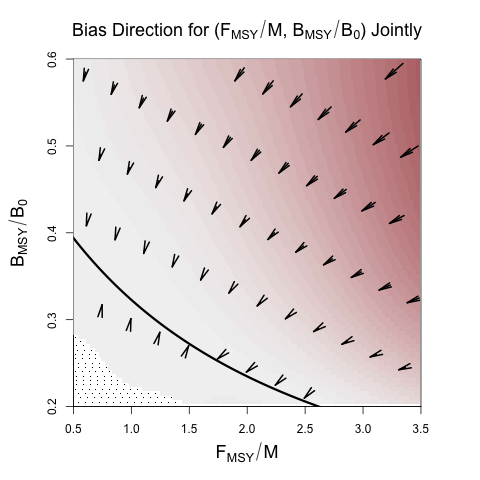
\includegraphics[width=0.48\textwidth]{../ddBias/directionalBiasDDSubExpT45N150A0-1AS4K0.2N38.png} %directionalBiasDDExpT45N150A0-1AS4K0.2.png}
%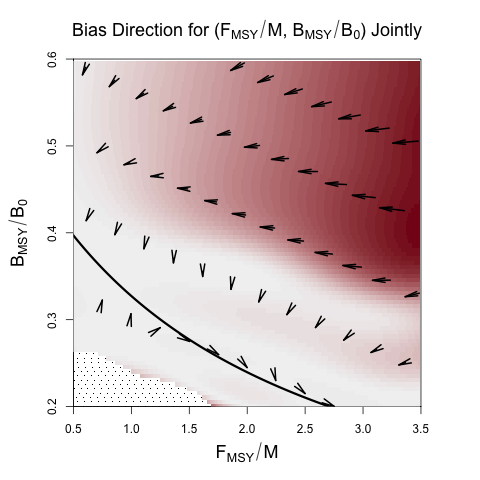
\includegraphics[width=0.48\textwidth]{../ddBias/directionalBiasDDSubFlatT45N150A0-1AS1K0.5N56.png} %../ddBias/directionalBiasDDSubFlatT45N150A0-1AS4K0.2N56.png} %94 %directionalBiasDDFlatT45N150A0-1AS4K0.2N28.png}
%\vspace{-0.75cm}
\caption{
RP mapping of BH DDM fit to Schnute DDM data under moderate growth ($a_s=1$ and $\kappa=0.5$).
$(left)$ High contrast simulation.
$(right)$ Low contrast simulation.
}\label{moderateGrowth}
\end{figure}

%\clearpage
%
The RP mappings seen in Figure (\ref{moderateGrowth}) show very similar RP mappings
to that of the SPM, with the biggest differences occurring
around the location of the break point where the low contrast model begins to
dramatically underestimate $\frac{F^*}{M}$.
%
In the high contrast simulation setting Figure (\ref{moderateGrowth}; $left$) shows
the RP mappings again demonstrate a similar nearly minimal distance mapping of
RPs onto the constrained BH RP set. In the low contrast setting Figure (\ref{moderateGrowth}; $right$) 
shows a very similar two regime pattern of RP inference is observed, however the
location of the break between these regimes appears at lower values of
$\frac{B^*}{\bar B(0)}$. In this moderate growth setting the break point
occurs around values of $\frac{B^*}{\bar B(0)}$ just below 0.4 as opposed to 
%\mbox{
the SPM where the break point occurs at values of $\frac{B^*}{\bar B(0)}$ just above 0.4.
%}

%\begin{itemize}
%\item largly the same as the production model limit.
%\item contrast is identical
%\item no contrast demonstrates the same general pattern, execept that the break point moves down so that less model misspecification is tolerated.
%\item break just below zeta=0.4
%\end{itemize}

%\clearpage
\subsection{Slow Individual Growth Dynamics\label{slow}}

%
The slow individual growth setting simulated here fixes $a_s=2$ and $\kappa=0.1$, to
simulate a species that grows quite slowly and matures into the reproducing  
stock relatively later than the previously describe simulations. This combination has 
the effect of exaggerating the components of the model dynamics which are related to
individual growth since individuals recruit at a smaller size and slowly
grow over the extent of the modeled period.

%
The slow growth of these dynamics oppose the simple production model setting
in the sense that they move the constrained RP set a large distance (largest
among the spectrum of decreasing $w(a_s)$ populations simulated here)
away from the $\frac{1}{x+2}$ limiting case. 
%It is interesting to note that
%this is true for all of the two parameter constrained constrained RP sets as
%seen in Figure (\ref{rpTriptic}).

%driven
Despite the heavily growth influenced biomass dynamics in this setting, 
the RP mappings seen in Figure (\ref{dramaticGrowth}) obviously bear a huge 
resemblance to the previously seen RP mappings. Again the biggest differences 
in the RP mappings occur around the location 
%of the break point where the low 
%contrast model begins to dramatically underestimate $\frac{F^*}{M}$.
%\clearpage
\begin{figure}[h!]
\begin{minipage}[h!]{0.44\textwidth}
%NOTE: REFINE
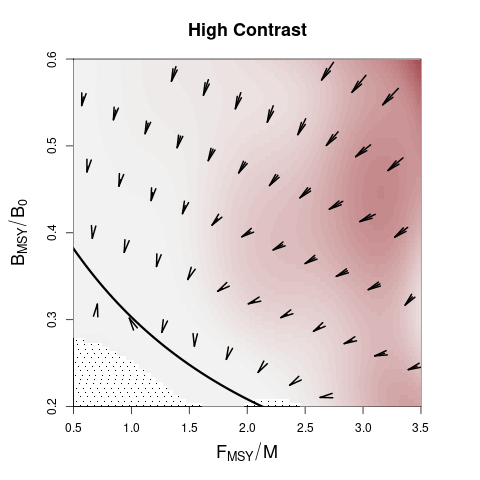
\includegraphics[width=\textwidth]{../ddBias/directionalBiasDDSubExpT45N150A0-1AS2K0.1Reds 2.png}
\end{minipage}
\begin{minipage}[h!]{0.44\textwidth}
%NOTE: change arrow spacing
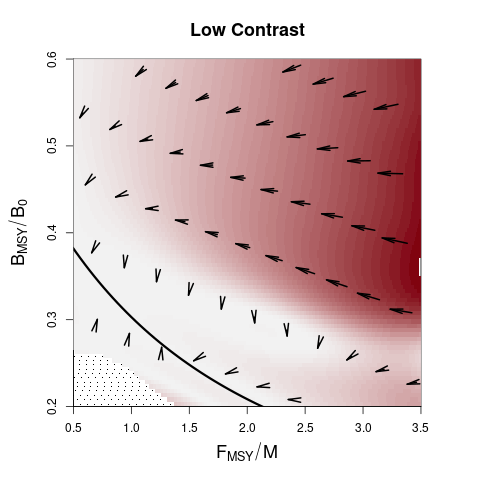
\includegraphics[width=\textwidth]{../ddBias/directionalBiasDDSubFlatT45N150A0-1AS2K0.1N84EdgeReds 2.png}
\end{minipage}
\begin{minipage}[h!]{0.09\textwidth}
\hspace{-1cm}
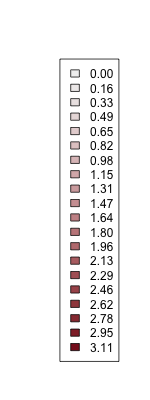
\includegraphics[width=1.5\textwidth]{../gpBias/legendSubSchnute.png}
\end{minipage}
%%\vspace{-0.5cm}
%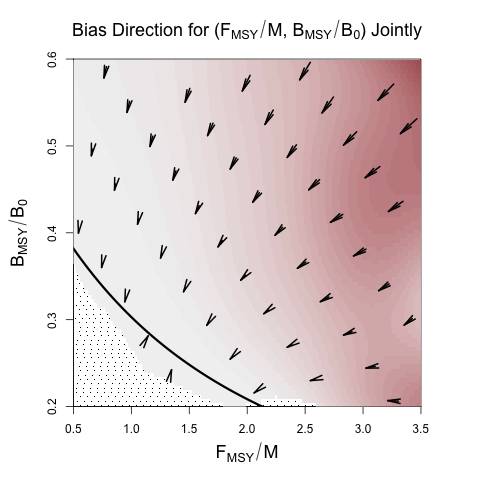
\includegraphics[width=0.49\textwidth]{../ddBias/directionalBiasDDSubExpT45N150A0-1AS2K0.1.png}
%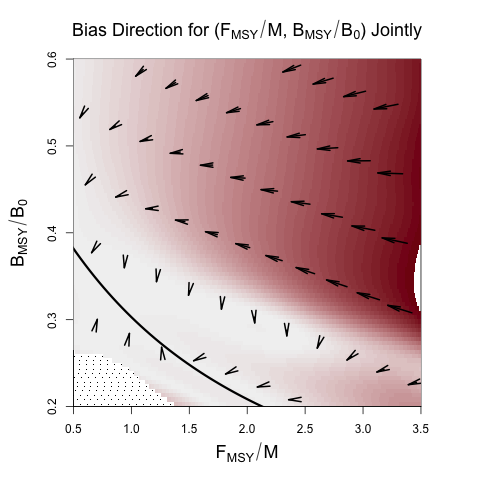
\includegraphics[width=0.49\textwidth]{../ddBias/directionalBiasDDSubFlatT45N150A0-1AS2K0.1N84Edge.png}
%\vspace{-0.5cm}
\caption{
RP mapping of BH DDM fit to Schnute DDM data under dramatic growth ($a_s=2$ and $\kappa=0.1$).
$(left)$ High contrast simulation.
$(right)$ Low contrast simulation.
}\label{dramaticGrowth}
\end{figure}
%\vspace{-0.5cm}
%
of the break point where the low contrast model begins to dramatically underestimate $\frac{F^*}{M}$.
%
In this low contrast setting the break point in RP estimation occurs around values of
$\frac{B^*}{\bar B(0)}$ well below 0.4 with the behavior extending as far down as 
\mbox{$\frac{B^*}{\bar B(0)}=0.3$}. This regime shift occurs well below that of the Ricker
set, as initially observed in the production model setting.
This reduced range of acceptable RP inference indicates that for slow growing stocks 
%under increasinglyemphatic growth
%\vspace{0.5cm}
%the model misspecification issue of the 
misspecified BH models becomes increasingly brittle with respect to RPs.
%to the simple production model where the break point occurs at $\frac{B^*}{\bar B(0)}$
%just above 0.4.

%
Interestingly this pattern only follows for the low contrast setting. In the high
contrast setting inference returns to a pattern resembling the minimal distance
mapping onto BH RP set, further pointing to the importance of contrast for informing
these models.

%\begin{itemize}
%\item introduce dramatic growth setting.
%
%\item extremely similar to the production model limit.
%\item contrast is identical
%\item no contrast demonstrates the same general pattern, execept that the break point moves down so that less model misspecification is tolerated.
%\item break well below zeta=0.4 as far down as 0.3
%\end{itemize}

%
%\clearpage
\subsection{Clustering Catastrophic Model Failure}

%%
%\subsection{Clustering Model Failure}

%
Considering the behavior observed in Sections (\ref{fast}-\ref{slow}), where
$\frac{F^*}{M}$ is dramatically underestimated, it is natural to ask
where specifically in RP space we might expect to see this catastrophic failure 
of the BH model as growth assumptions change.
%
%The structure of RPs under the BH model suggests several potential avenues for
%forming hypotheses to identify highly misspecified RP regions. 
%however identifing cases where $\frac{F^*}{M}$
%but the single
%clearest feature to identify are cases where $\frac{F^*}{M}$ is
%heavily under-estimated. 
%Here a hypothesis testing inspired framework is used to identify these cases.
%By using the GP metamodel to propagate estimate uncertainty across the simulated 
%RP space the metamodel can predict which stocks may fail when modeled under 
%the BH model. 
Below a hypothesis testing inspired classifier is derived in terms of the GP predictive structures 
for identifying where BH inference fails in this way. 
%% of misspecified BH RPs.
%%as a surrogate for the distribution of 
%%$\frac{F_{MSY}}{M}$ across degrees of misspecified BH models. 
%This allows for a rejection threshold (against the null hypothesis that BH RP
%estimates are unbiased) to be derived in terms of the GP predictive structures
%to define a classifier for identifying where BH inference breaks down
%broadly over RP space.


%\clearpage
%
Recall that the metamodel models MLEs of $log(F^*)$ under the misspecified BH model.
%is a metamodeled quantity, 
%corresponding to $$, $log(F_{MSY})$, corresponding to is the metamodeled 
Thus, for a given predictive set of RPs, $\textbf{x}^\star$, the BH metamodeled
quantity is given by kriging prediction as $N(\hat y(\textbf{x}^\star), \hat \sigma^2(\textbf{x}^\star))$,
where $\hat y(\textbf{x}^\star)$ is the kriging mean (as previously described in
Eq. (\ref{gpYHat})) and $\hat \sigma^2(\textbf{x}^\star)$ provides estimate
uncertainty via the kriging predictive variance given by,
\begin{equation} %k(x) a n−vector with kν,j (x) = K(x, xj ), for all xj ∈ X
       \hat \sigma^2(\textbf{x}^\star) = \textbf{R(x}^\star, \textbf{x}^\star\textbf{)} - \textbf{r(x}^\star\textbf{)}'\bm{R}^{-1}_{\bm{\ell}}\textbf{r(x}^\star\textbf{)}.
\end{equation}

%
Model failure with respect to estimating $\frac{F^*}{M}$ under the BH
model is measured by the percent error as previously described in Section (\ref{highConRes}).
When the BH model estimates $\frac{F^*}{M}$ well, the percent error is
expected to be small in the following sense,
%In this setting to define the degree of model failure the percent error of the 
%estimate is capped at no more than $P$ 
%with respect to $\frac{F_{MSY}}{M}$ 
%the percent error is capped to 

%
\begin{equation}
\frac{\frac{F^*}{M}-\frac{\hat{F}^*}{M}}{\frac{F^*}{M}}\le P. \label{pError}
\end{equation}

%
$P$ defines the extent of model failure on the scale of percent error. For
measuring catastrophic model failure $P$ was chosen to be $0.5$, but smaller values
of $P$ may be chosen to emphasize regions of more subtle model failure. %subtle regions 
%
Since $\frac{F^*}{M}$ is generally underestimated for stocks above the BH set, a 
one-sided test is used to identify model failure.
Thus, when the percent error is statistically greater than $P$ the notion that
the BH model estimates $\frac{F^*}{M}$ well (in the sense defined by $P$) is rejected.

%
For statistical evaluation, it is convenient to rearrange Eq. (\ref{pError})
as \mbox{$\hat{F}^*\ge (1-P)F^*$}. $\hat{F}^*$ is then distributed as $LN(\hat y(\textbf{x}^\star), \hat \sigma^2(\textbf{x}^\star))$,
and catastrophic model failure is predicted
%the notion that BH RP estimates are well estimated 
%is rejected for  
%rejection region (against the  that BH RP
%estimates are unbiased) is then defined as the RPs for which the $5^{th}$ percentile
in regions of RP space where the $5^{th}$ percentile of the 
Log-normal distribution falls below \mbox{$(1-P)F^*$.}

%\clearpage
\begin{wrapfigure}{r}{0.50\textwidth}
%\vspace{-1.1cm}
%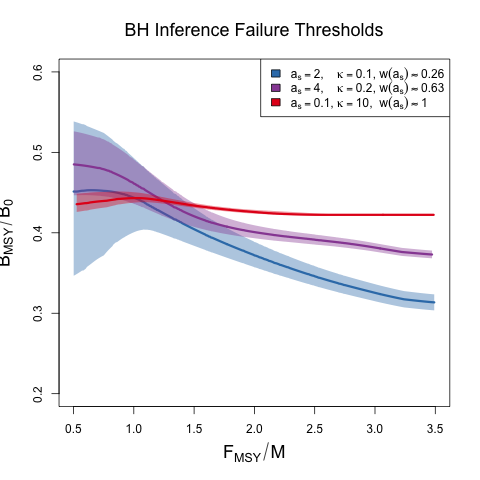
\includegraphics[width=0.45\textwidth]{../ddBias/metaLowerZetaLinesDDFlatT45N150A0-1AS2K0.1N84Edge.png}
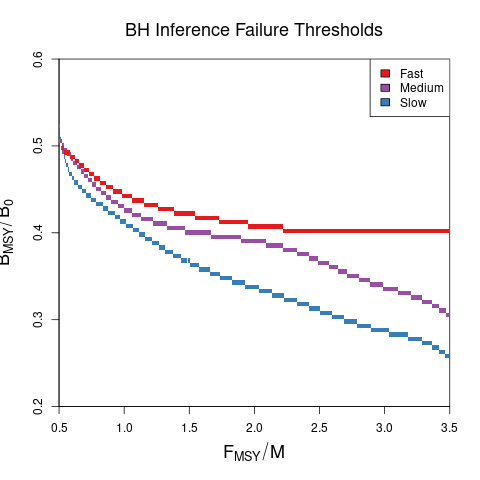
\includegraphics[width=0.45\textwidth]{../ddBias/relErrorImagesBHDD0.5.png}
%%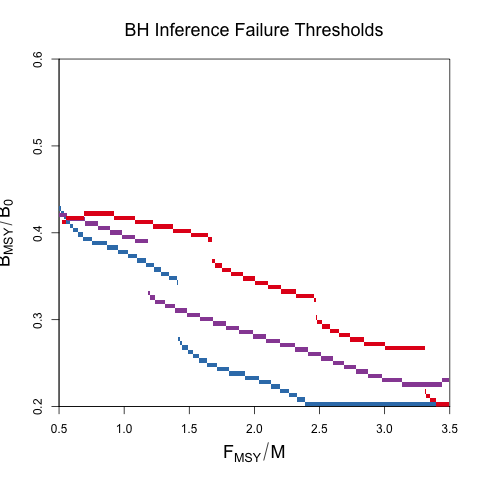
\includegraphics[width=0.45\textwidth]{../ddBias/relErrorImagesBHDD0.2.png}
%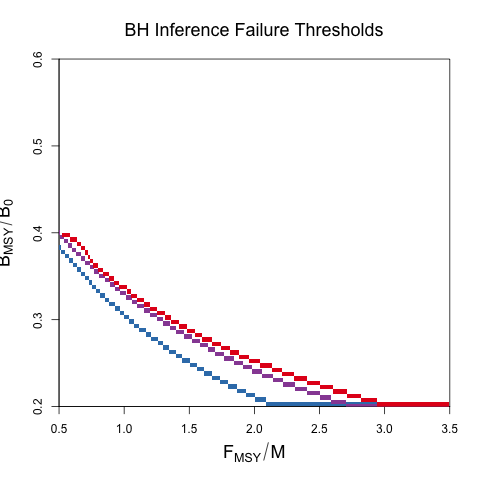
\includegraphics[width=0.45\textwidth]{../ddBias/relErrorImagesBHDD0.01.png}
\vspace{-0.5cm}
\caption{BH RP estimation catastrophic model failure ($P=0.5$) thresholds with decreasing individual growth dynamics.
}\label{breaks}
\end{wrapfigure}

%%
%Figure (\ref{breaks}) shows the rejection thresholds for the low contrast
%simulations of each of the fast, medium, and slow growth simulation settings. %emphatic, moderate, and no growth settings. %, moderate growth, and emphatic growth 
%The lines represent the estimated 
%%with a false positive rate of about 15\%, and the light shaded regions show how the rejection threshold
%%changes as the false positvie rate rages from 50\% to 2.25\%.
%When applied to the high contrast simulations the rejection threshold falls
%outside of the simulated RP range as expected by inspection of the
%high contrast RP mappings.
%%Figures (\ref{}) is outside the range of  The rejection threshold as applied to the high contrast models does not  
%
%%
%Notice in Figure (\ref{breaks}) that the rejection threshold is subject to two
%axese of sensativity. Firstly, for each simulated growth the rejection
%threshold is more sensative for small values of $\frac{F_{MSY}}{M}$ than for
%large values. This is a natural result since discerning $\hat y(x)$ below the
%minimum simulated RP becomes more difficult when the data are truely generated
%near the minimum simulated $\frac{F_{MSY}}{M}$.
%%as those values $\hat y(x)$ from $\theta_{min}$ has maximum overlap at $\theta_{min}$
%For large $\frac{F_{MSY}}{M}$ the minimum distance mapping results in $\hat y(x)$
%well above the minimum simulated RP but for small $\frac{F_{MSY}}{M}$ even the
%minimum distance mapping may be close to the rejection threshold.
%
%%
%The second axis of sensativity is between individual growth simulations.
%The no growth setting produces a very clear threshold of model failure, while
%the failure threshold for emphatic growth is much more varied, especially near
%the minimum simulated $\frac{F_{MSY}}{M}$. % setting appears to be less certain about     
%This is largely due to the increased RP estimate uncertainty as growth becomes
%more emphatic in the dynamics.

%Nick will describe the results in Figure (\ref{breaks}). Probably keep it short. Maybe a page.
Figure (\ref{breaks}) shows the clustering thresholds for the low contrast
simulations of each of the fast, medium, and slow growth simulation settings.
%$P=0.5$
%Clustering thresholds shown here are calculated for catastrophic model failure 
%as defined by $P=0.5$.  
Each line separates hypothetical stocks where simulations would expect the BH model %to experience 
to catastrophically fail in RP estimation. % model failure when modeled with a BH model, such that stocks above each 
A percent error of 50\% was chosen to represent the threshold of catastrophic model failure so that the 
nearly minimal distance mapping
%shortest distance mapping 
occurs below the lines and dramatic underestimation of $\frac{F^*}{M}$ occurs for data generated
above each line.

%$P=0.5$ was chosen to represent the threshold between the shortest distance mapping and 
%Below each line RP estimation of the BH model is less that 50\% percent bias and above each line the  mapping is shortest distance and above the line the 
%mapping represent catestrophic model failure of the BH model. The line represents the threshold where 
%statistically the behavior changes.

%
In general clustering thresholds are oriented to the shape of the BH RP set in each of the simulated individual 
growth settings. As individual growth slows from the SPM limit (in red) to the most emphatically slow growing 
simulation in blue, the BH model fails catastrophically for an increasingly large range of RP space. 
This indicates that the slower growing simulation makes the BH model more brittle to model misspecification. 
In particular the fragility of the BH model is exacerbated most for high $\frac{F^*}{M}$ stocks as individual growth slows. %stocks in the slower individual growth setting 
For low $\frac{F^*}{M}$ stocks the failure thresholds for each simulated individual growth setting %seems to 
converges around the common value $\frac{B^*}{B_0}=0.5$.

%Overall the misspecified BH model in the slower growth setting is more brittle than for faster growing settings.

%
Model misspecification of the BH model is compounded in the slower individual 
growth settings, indicating an interaction between the functional form of 
recruitment and growth dynamics. In the following section, this interaction is 
exemplified by exploring oscillatory dynamics that arise outside of the more 
biological regimes explored here.
%interact with growth dynamics to produce 
%unique behaviors as exemplifiedin Section (\ref{oscillation}).

%\clearpage

%\begin{itemize}
%%\item $\alpha_0\approx0.16$$\alpha_0\in[0.5, 0.0225]$ shows
%%\item clustering is more uncertain for small $F_{MSY}/M$ since differentiating 
%%$\hat y(x)$ from $\theta_{min}$ has maximum overlap at $\theta_{min}$.
%%\item no growth is more certain than emphtic growth, since estimates under the 
%emphatic growth setting are more uncertain leading to more overlap between infence classes.
%\item a general statement about the range of the rejection threshold
%\end{itemize}

%\clearpage
\subsection{Oscillatory Growth. The Road to Chaos.\label{oscillation}}

%%
%While the above patterns of RP estimation follow for biologically inspired 
%growth patterns (i.e. $corr(a_s, \kappa)<0$),
While the above patterns of RP estimation follow for the negatively correlated 
growth and maturity parameters (i.e. $corr(a_s, \kappa)<0$),
%of the $w(a_s; \kappa)=c$ level curve,                  biological
as $a_s$ increases to weaken (and eventually reverse) this negative 
correlation between $a_s$ and $\kappa$, a regime of oscillatory dynamics appear. %also exists within these dynamics. 
While RP estimation behaves somewhat similar in this oscillatory regime there 
are unique features in this setting. 
%that are not present in the more biological regimes. 
Below consider the oscillatory example of a logistic DDM with 
$a_s=10$, $\kappa=0.1$ and fishing fixing at $F^*$ (i.e. low contrast: $\chi=0$).
%Moderate w(a_s)\approx0.6

%{\color{red} maybe an appendix}
\begin{figure}[h!]
\centering
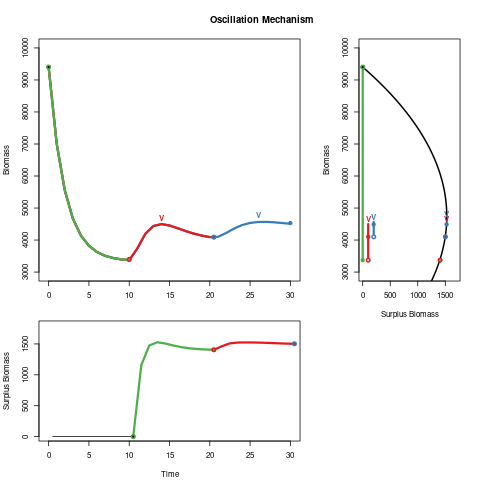
\includegraphics[width=0.85\textwidth]{../ddBias/shockBiomassSurplus.png}%Yeild.png}
\vspace{-0.5cm}
\caption{$top~left:$ Logistic DDM biomass over 30 epochs of time with $a_s=10$.
Green, red, and blue colors indicate three 10 epoch long windows of biomass.
v indicates local biomass oscillation maxima.
$top~right:$ %Yield 
Surplus biomass production plotted over the range of biomasses shown.
The biomass range of each 10 epoch window is shown in the vertical colored lines.
$bottom~left:$ %Yield 
Surplus biomass production plotted through time. Colors correspond to the
lagged biomass region that results in the evaluated yield. The black horizontal
line demonstrates the pre-model assumption of biomass fixed at $B_0$.
}
\label{shock}
\end{figure}

%
\clearpage

%
Figure (\ref{shock}) demonstrates the mechanism of how these oscillatory
dynamics form. Oscillatory dynamics appear when fishing pushes biomass past
$B^*$ within the lagged $a_s$ window. %of recruitment. 
When $t\le0$ the delay model assumes that biomass is fixed in equilibrium at $B_0$. 
Therefore in the green region of the biomass series, $0<t<10$, the population recruits 
at $R(B_0)$. Figure (\ref{shock}) shows that in this initial period $R(B_0)$ results in 
zero surplus yield for that period, and biomass falls as a result.

%
Once $t$ exceeds $a_s$, the lagged recruitment refers to the integrated
biomass series to evaluate recruitment based on $B_{t-a_s}$. The red
region of the biomass series is the result of surplus biomass production 
(i.e. evaluation of the yield curve) %yield 
over the initial green biomasses. Figure (\ref{shock}) shows that the %yield 
surplus biomass production over the green biomass series first increases, 
as biomass decreases to approach $B^*$ ($B^*\approx5000$ here). As biomass 
decreases below $B^*$, surplus biomass then decreases to create
%and then decreases as the biomass crosse $B_{MSY}$. This creates 
the local maximum in the red biomass series.

%
Furthermore, the blue region of the biomass series is then based on surplus biomass %yield
over the red biomasses. Notice that since the red biomasses first increase and
then decrease, surplus biomass %yield 
increases as the red biomass increases and surplus biomass subsequently decreases  %toward$B^*$, and yield subsequently decreases 
following the descending leg of the red biomass series. This %yield%in the oscillation of the red biomass series. 
surplus biomass pattern carries the oscillation of the red biomass region
forward into the blue region despite the red biomasses never increasing past $B^*$. 
%Each crossing of $B^*$, as may be forced by fishing, created a compounding oscillatory component.

%
This process of biomass oscillation carries on in this manner nonetheless
approaching equilibrium at $B^*$. Equilibrium is reached in an oscillatory
manner set off by the green biomass series crossing over from above $B^*$
to below it. The example shown in Figure (\ref{shock}) exemplifies the oscillatory 
phenomena simulated here, but the mechanism that produces these oscillations may
occur with other forms of recruitment, or fishing, outside of logistic recruitment 
whenever fishing causes biomass to cross over $B^*$ within the lagged recruitment 
window. By repeatedly forcing the population biomass over the $B^*$ threshold, in 
this manner, the dynamics can quickly resemble the behavior of chaotic equations \cite{ausloos_logistic_2006, sprott_simple_2007}. %ticresembling that of chaotic 

%
\subsubsection{RP Estimation}

%
Statistical inference in the oscillatory regimes of individual growth can be 
challenging. Depending on the parameters inferred, the likelihood can have 
multiple local modes which require global optimization techniques to distinguish. 
Furthermore, parameter estimation is more uncertain in this setting as the 
likelihood may confuse oscillations with residual noise.
%This uncertainty extends to RP estimation, high contrast setting, $w\approx0.6$ $a_s=10$

%Figure (\ref{oscillationArrow}) shows the BH RP mapping fixing $w(10;0.1)\approx0.6$
%in the high contrast simulation setting. This places the 
%dynamics firmly in the ocillatory regiem, but the high 
%contrast setting provides significant information for inferring recruitment parameters.
%
%\clearpage
%\vspace{-1cm}

%high 
Figure (\ref{oscillationArrow}) shows the BH RP mapping fixing $w(10;0.1)\approx0.6$
in the high contrast simulation setting. This places the
dynamics firmly in the oscillatory regime, but the high 
contrast setting provides significant information for 
inferring recruitment parameters.

%
\clearpage
\begin{wrapfigure}{r}{0.50\textwidth}
%\vspace{-1.25cm}
%\vspace{-1.15cm}
\begin{minipage}[h!]{0.92\textwidth}
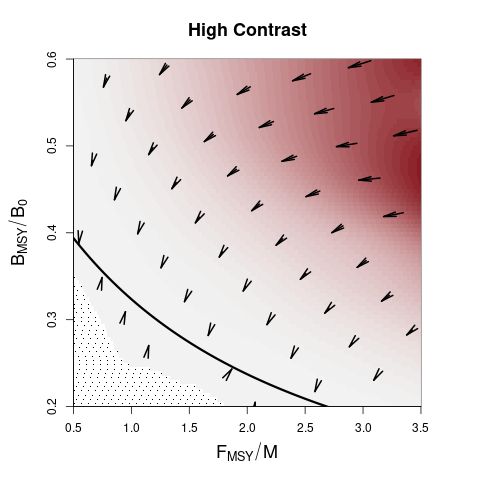
\includegraphics[width=0.49\textwidth]{../ddBias/directionalBiasDDSubExpT45N300A0-1AS10K0.1Reds 2.png}
\end{minipage}
\begin{minipage}[h!]{0.06\textwidth}
\vspace{-7cm}
\hspace*{6cm}
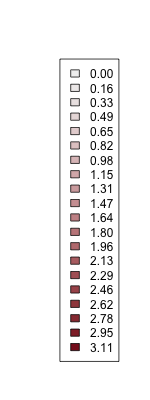
\includegraphics[width=1.7\textwidth]{../gpBias/legendSubSchnute.png}
\end{minipage}

\vspace{-0.75cm}
\caption{RP mapping of BH DDM fit to high contrast Schnute DDM data under oscillatory growth ($a_s=10$ and $\kappa=0.1$).
}\label{oscillationArrow}
\end{wrapfigure}

%
Interestingly in this high contrast setting, a very similar two regime pattern
of RP inference is observed as previously seen in low contrast settings.
That said the boundary between the regimes in this setting is much smoother
%DISCUSISON: due to more uncertain modes smoothly changing 
and the location of the break between these regimes appears around higher values of
$\frac{B^*}{\bar B(0)}$. %of HIGHER values.

%%
%\begin{wrapfigure}{r}{0.50\textwidth}
%\vspace{-1cm}
%\centering
%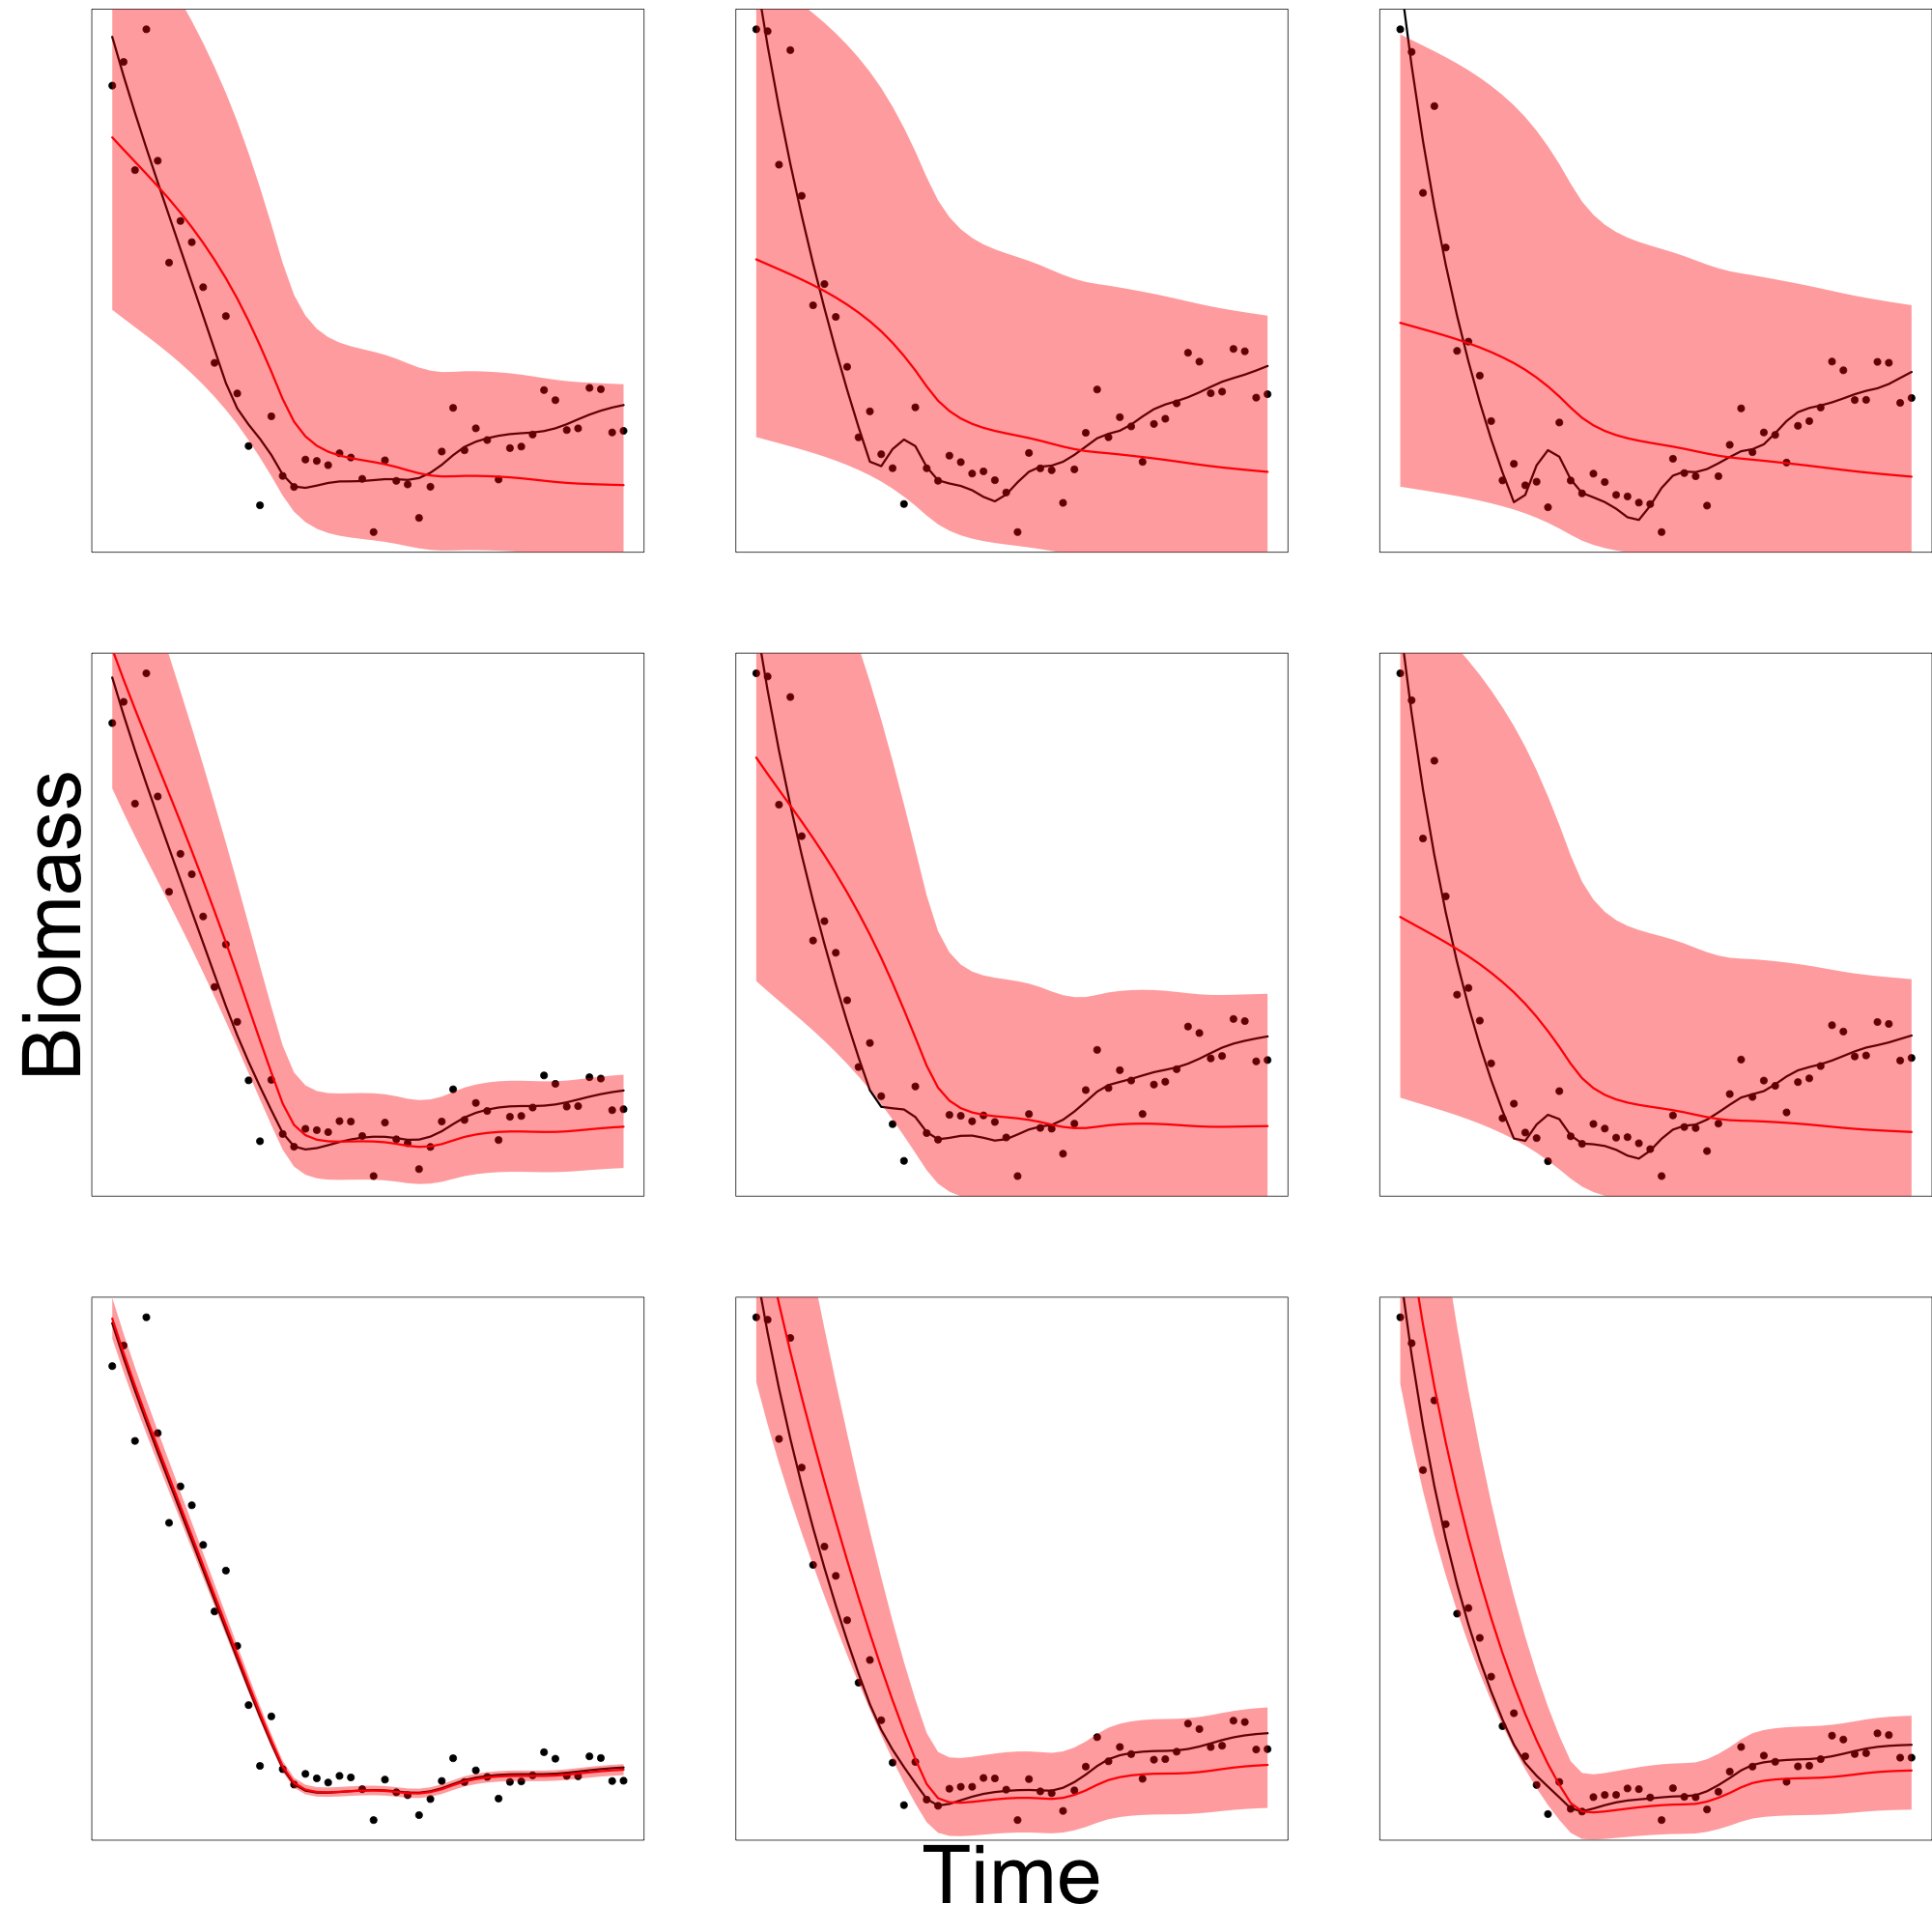
\includegraphics[width=0.45\textwidth]{../ddBias/indexGridExpT45N300A0-1AS10K0.1.png}
%\vspace{-0.45cm}
%%\begin{tikzpicture}[overlay]
%%\node at (5,-0.5) {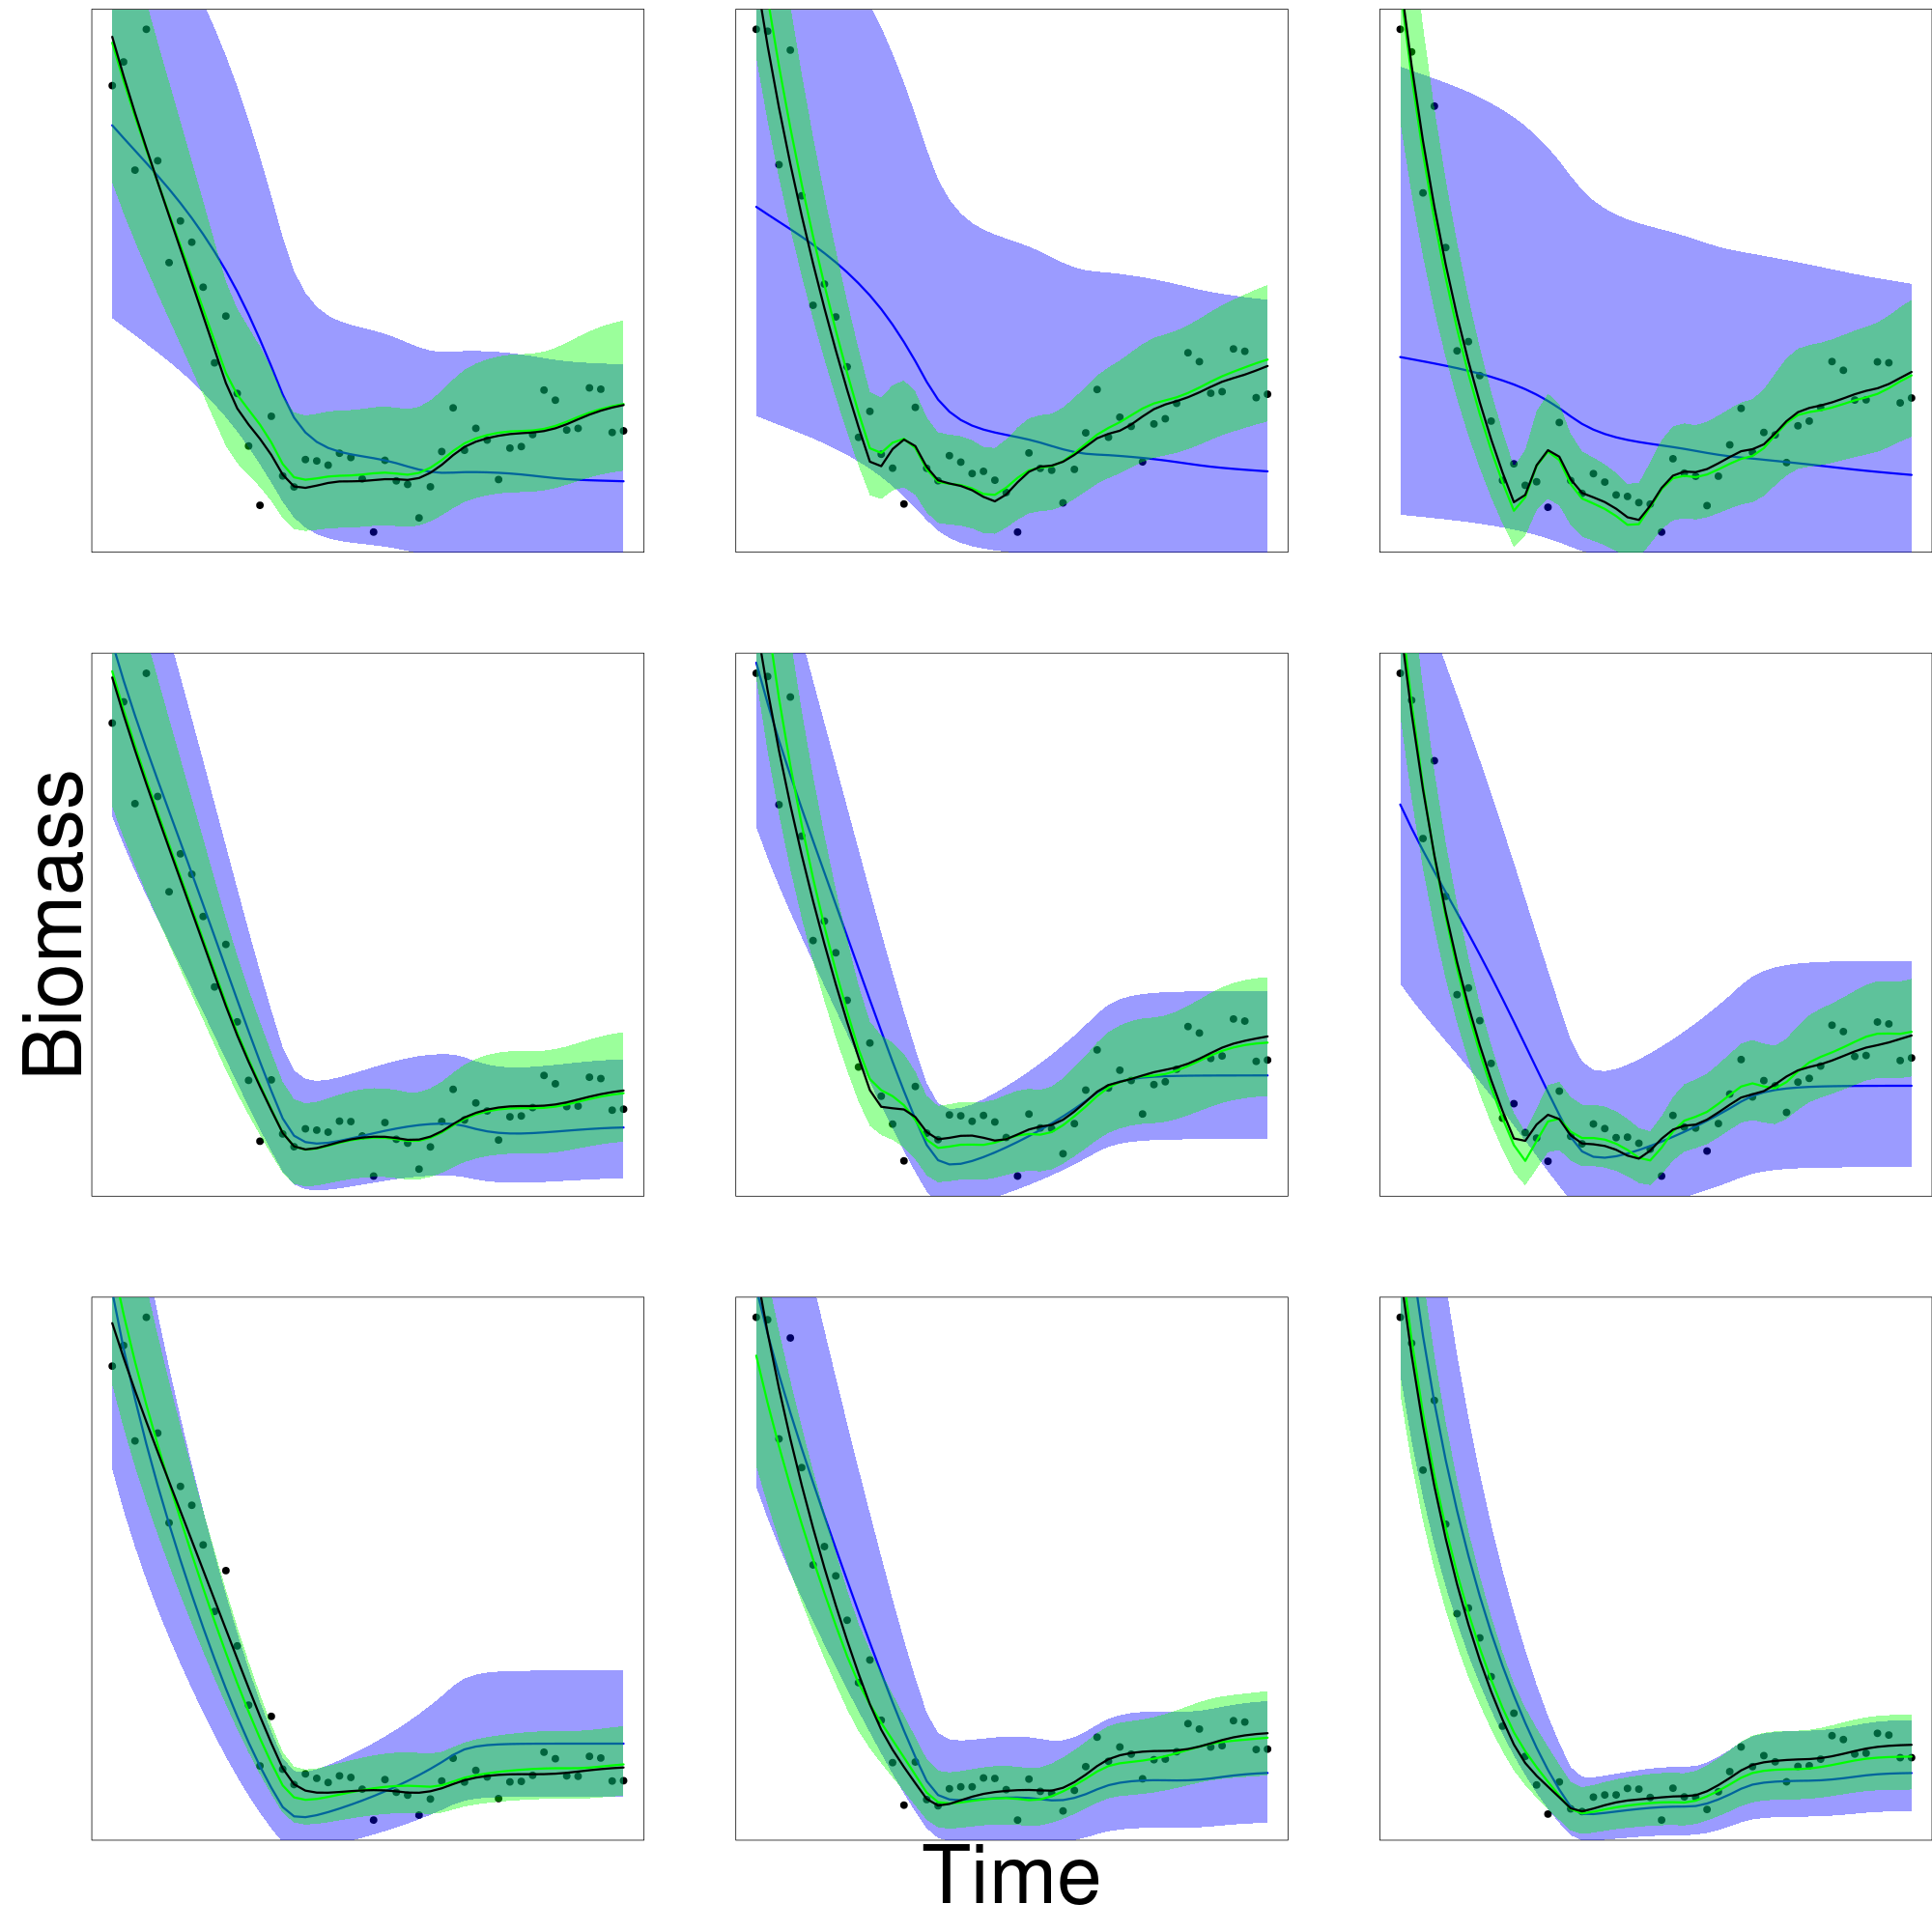
\includegraphics[width=0.49\textwidth]{../ddBias/indexGridKAExpT45N300A0-1AS10K0.1.png}};
%%\node[minimum size=7, inner sep=-2] at (5,-3.5){Time};
%%\node[minimum size=7, inner sep=-2, rotate=90] at (2,-0.5){Biomass};
%%}
%%\end{tikzpicture}
%\caption{Example BH fits ($red$) to Schnute data ($black$). Each example plot is arranged to mirror its location in RP space.
%%Higher $\frac{B^*}{\bar B(0)}$
%%is arranged higher veritically, and higher $\frac{F^*}{M}$ is arranged farther 
%%to the right horizontally so as to mirror the RP space domain. 
%}\label{bhGrid}
%\end{wrapfigure}

%
This higher $\frac{B^*}{\bar B(0)}$ break point, hovering around 0.5, is
consistent with the mechanism which induces oscillation. 
%When the initial contion of biomass is started at $B_0$Starting the biomass
%at $\bar B(0)$ in the ocillatory regiem, 
For fixed $B_0$ increased $\frac{B^*}{\bar B(0)}$ will tend to exacerbate oscillatory behavior 
by increasing $B^*$ so that biomass is more easily pushed past $B^*$ by fishing
within the initial lagged window of recruitment. This produces more dramatic 
oscillations in the higher $\frac{B^*}{\bar B(0)}$ region of RP space. This 
phenomena may also be understood in terms similar to the notion of elasticity 
described by Yeakel and Mangel \cite{yeakel_generalized_2015} and its relationship 
with $\gamma$ and $B^*$.
%Similarly this phenomena may be understood in terms of the relationship between $\gamma$, 
%$B^*$, and the notion of elasticity described by Yeakel and Mangel \cite{yeakel_generalized_2015}.

%\begin{itemize}
%\item RP estimation is harder when ocilations are present
%\item Ocillations may be confused with noise.
%\item $w\approx0.6$ $a_s=10$
%\item Here the high contrast simulation setting is shown.
%\end{itemize}
%

%
\clearpage

%
\begin{wrapfigure}{r}{0.50\textwidth}
%\vspace{-0.75cm}
\centering
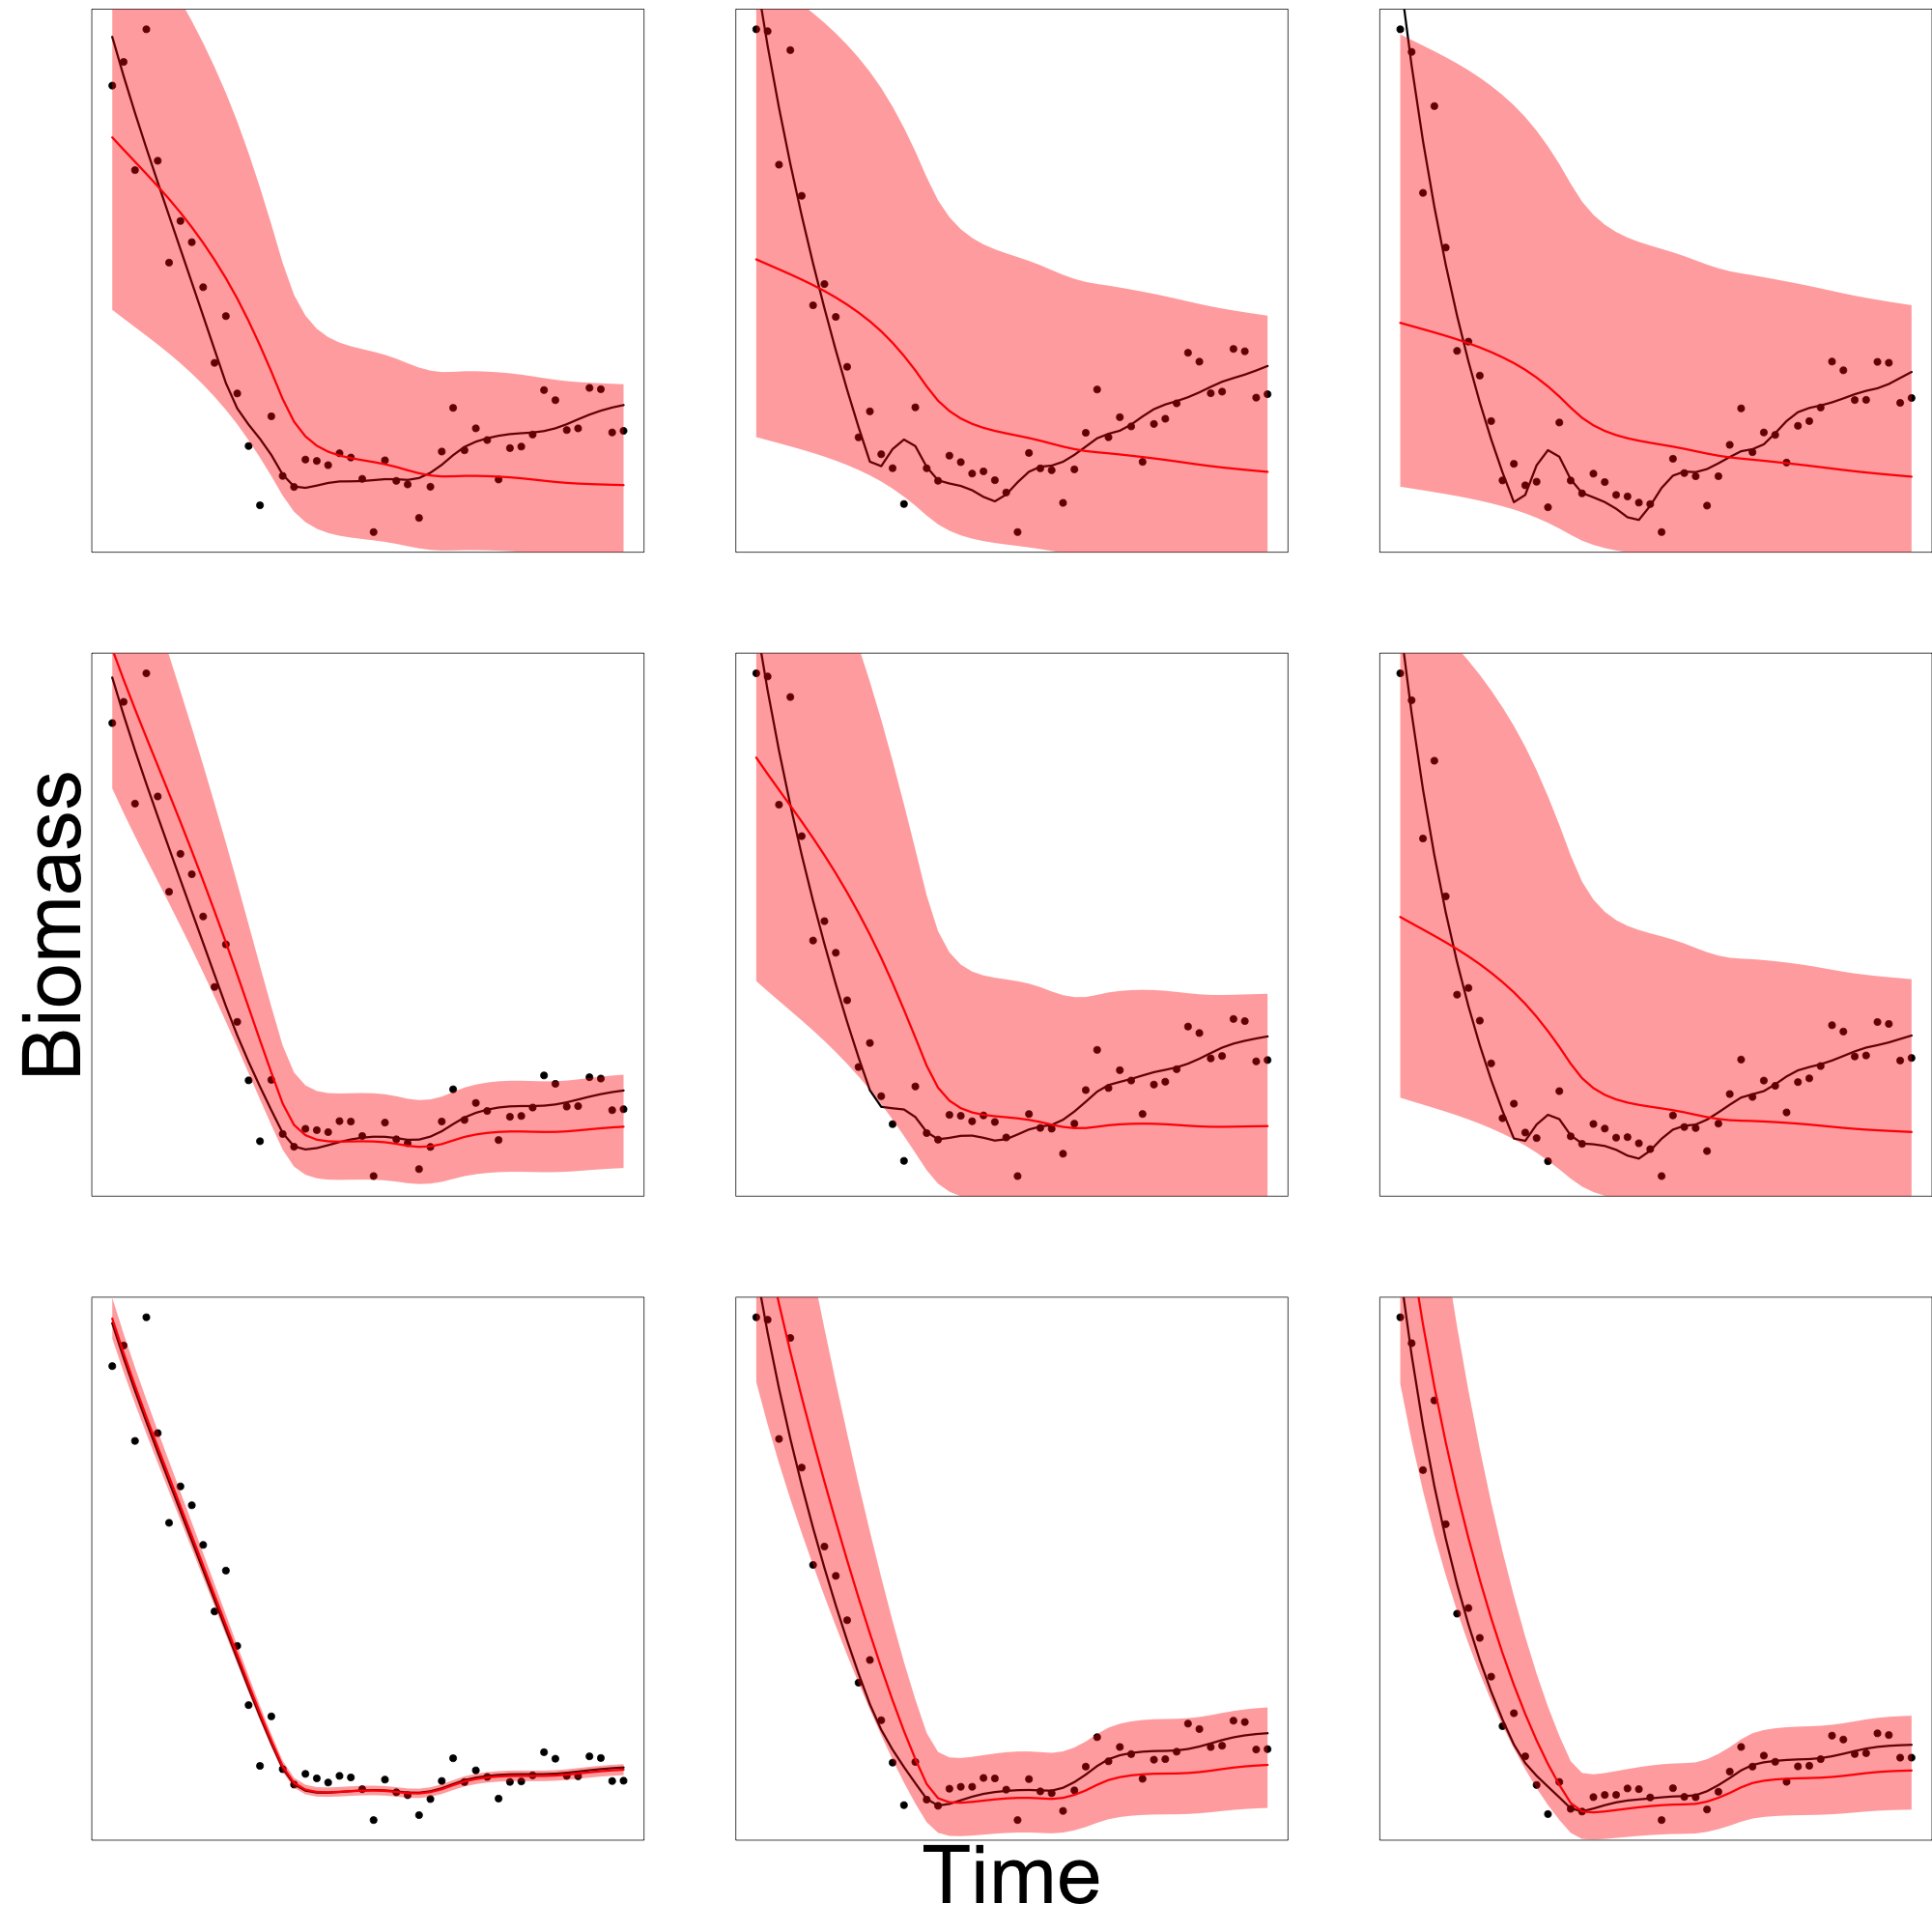
\includegraphics[width=0.45\textwidth]{../ddBias/indexGridExpT45N300A0-1AS10K0.1.png}
\vspace{-0.45cm}
%\begin{tikzpicture}[overlay]
%\node at (5,-0.5) {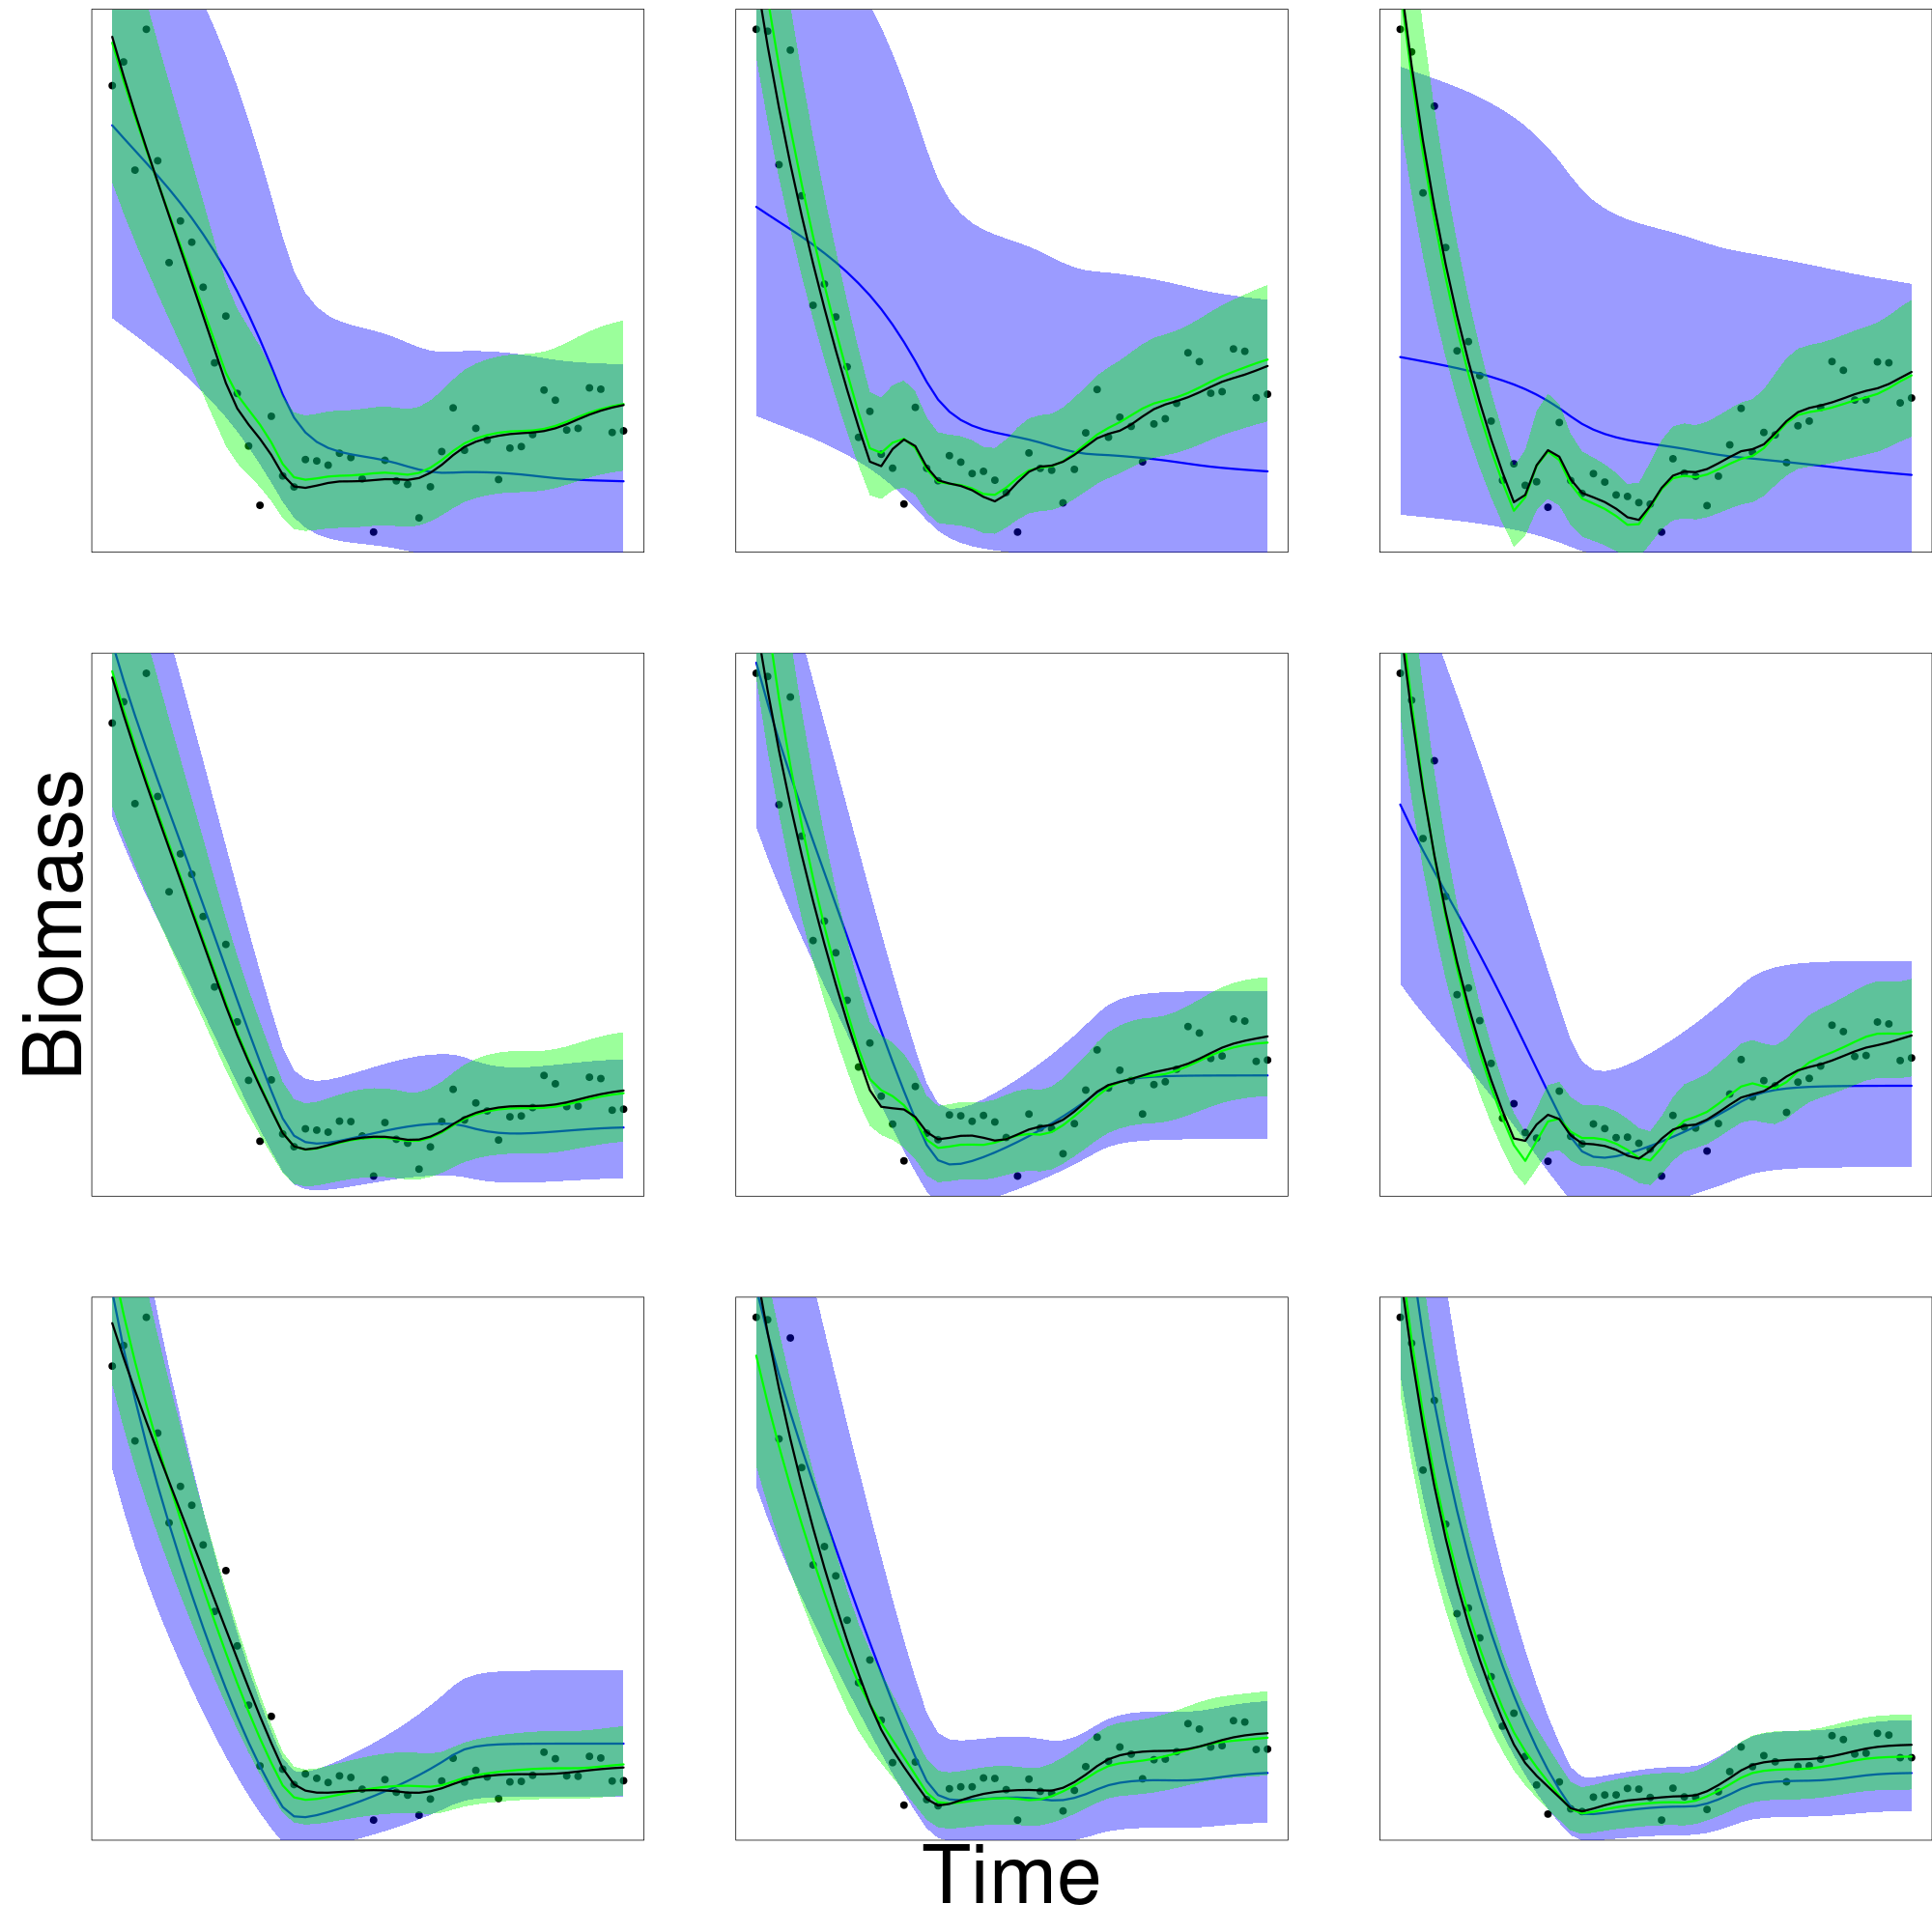
\includegraphics[width=0.49\textwidth]{../ddBias/indexGridKAExpT45N300A0-1AS10K0.1.png}};
%\node[minimum size=7, inner sep=-2] at (5,-3.5){Time};
%\node[minimum size=7, inner sep=-2, rotate=90] at (2,-0.5){Biomass};
%}
%\end{tikzpicture}
\caption{Example BH fits ($red$) to Schnute data ($black$). Each example plot is arranged to mirror its location in RP space.
%Higher $\frac{B^*}{\bar B(0)}$
%is arranged higher veritically, and higher $\frac{F^*}{M}$ is arranged farther 
%to the right horizontally so as to mirror the RP space domain. 
}\label{bhGrid}
\end{wrapfigure}

%
The fitted BH model does not produce significant oscillations because
under the BH model $\frac{B^*}{\bar B(0)}$ is constrained below 0.5 with the
majority of the simulation BH $\frac{B^*}{\bar B(0)}$ RPs falling between 0.4 and 0.2. % in the simulated RP domain. 
Therefore, the fitted BH model will not tend to push biomass past $B_{MSY}$ and
thus is incapable of modeling oscillatory biomass series. Figure (\ref{bhGrid})
shows a subset of example BH fits, which demonstrates the limited oscillatory
capacity of the BH fits. Furthermore, since the BH model has a limited
oscillatory capacity in this setting, the BH model tends to explain the
oscillations with artificially high residual variation and artificially low
%steepness 
$\alpha$, focusing fits on overly simplistic trends in the data.

%\begin{itemize}
%\item RP inference breaks in a simplifing manner as previously described
%\item breaks for high $\frac{B_{MSY}}{B_0}$, max model misspecification, also more ocilation due to mechanism.
%\item modeling with BH forces a low $\frac{B_{MSY}}{B_0}$ which cannot produce ocilations over the simualated biomass range.
%\item Thus when oscilations become a dominant effect the BH model focuses on fitting the overall trend with low steepness  
%\end{itemize}


%
\subsubsection{Estimating More\label{estMore}}

%
Figure (\ref{estAK}) shows a subset of example model fits to Schnute data 
simulated broadly over RP space with residual variation, $\sigma=0.12$, 
resulting in a CV of about 6\%.
Model fits are shown both under the two-parameter BH model as well as under the
three-parameter Schnute model, each model estimating all of its recruitment parameters  
as well as the individual growth and maturity parameters $\kappa$ and $a_s$.
%Notice that the BH model, even when additionally estimating $\kappa$ and $a_s$,
%does not gain the flexibility to properly model Schnute data.
%\begin{figure}[h!]
\begin{wrapfigure}{r}{0.50\textwidth}
%\vspace{-1.15cm}
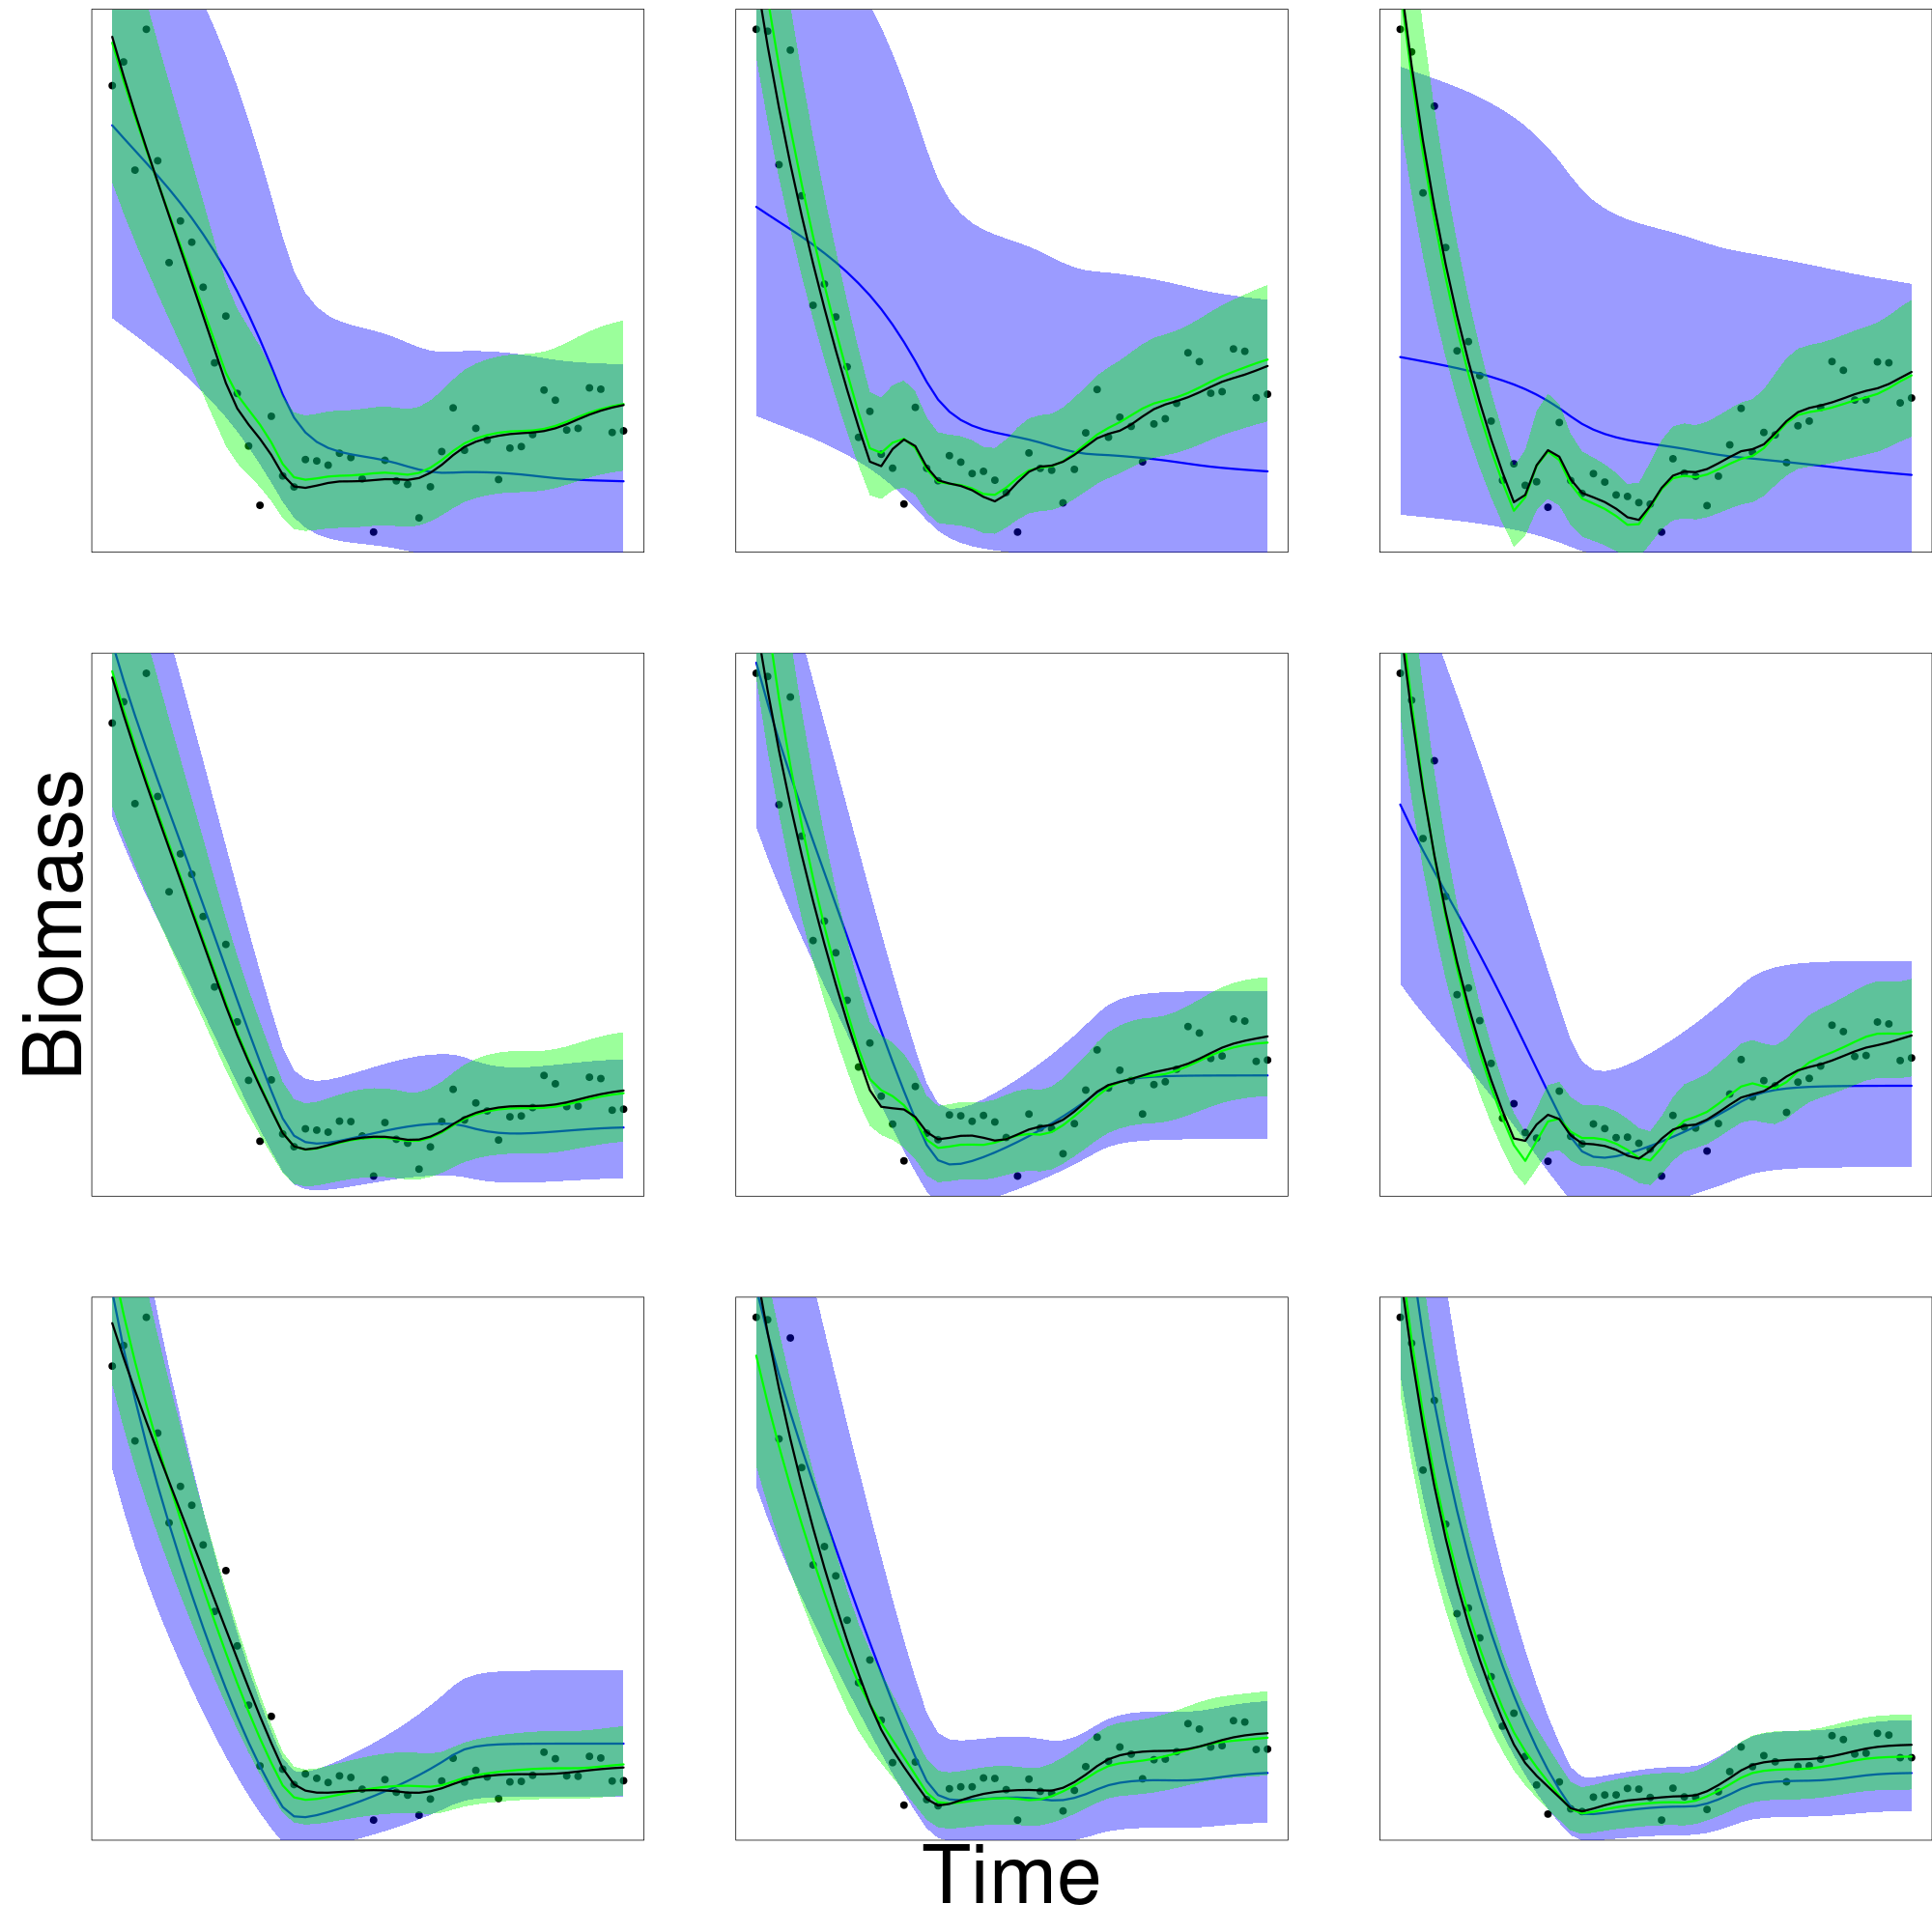
\includegraphics[width=0.49\textwidth]{../ddBias/indexGridKAExpT45N300A0-1AS10K0.1.png}
%\vspace{-0.5cm}
\caption{
$\kappa$ and $a_s$ estimation under BH ($blue$) and Schnute ($green$) fits to
Schnute data ($black$) arranged to mirror RP space. %Each model additionally estimates $\kappa$ and $a_s$.
%Higher $\frac{B^*}{\bar B(0)}$ is arranged higher veritically, and higher $\frac{F^*}{M}$ is arranged farther
%to the right horizontally so as to mirror the RP space domain.
}\label{estAK}
%\end{figure}
\end{wrapfigure}
%%
%Figure (\ref{estAK}) shows a subset of example model fits broadly over RP space.
%Model fits are shown both under the two-parameter BH model as well as under the
%three-parameter Schnute model, each model estimating all of its recruitment parameters as 
%well as the individual growth and maturity parameters $\kappa$ and $a_s$.
While estimating $\kappa$ and $a_s$ is not typically done in practice, these 
parameters are estimated here to demonstrate the interaction that can be present 
between recruitment and growth parameter estimation. Notice that the BH model, even 
when additionally estimating $\kappa$ and $a_s$, does not gain the flexibility 
to properly model Schnute data.

%
On the one hand the lack of oscillatory dynamics produced by the BH model causes the misspecified
BH fits in Figure (\ref{estAK}) to largely estimates $\kappa$ and $a_s$ so as to
approximate the SPM limiting case. The fitted Schnute model on the other hand, can 
produce the oscillatory dynamics and thus the information in the oscillatory data
well inform estimates of $\kappa$ and $a_s$ under the Schnute model. Furthermore,
the Schnute model has no issue learning its $\gamma$ parameter.
%for largely misspecified BH models.Figure (\ref{bhGrid}).  
%%
%\begin{itemize}
%\item Estimate $a_s$, $\kappa$ with BH => still results in the same inferential pattern (cannot learn $a_s$, $\kappa$)
%\item Estimate $a_s$, $\kappa$ with Schnute => not only fixed the inferential patter (can learn $\gamma$) but also can learn $a_s$, $\kappa$
%\item 
%\end{itemize} 

%
While statistical inference in the oscillatory regime can be challenging in
the highly constrained BH model, the Schnute model can easily estimate its extra
$\gamma$ parameter. The flexibility of estimating $\gamma$ simplifies inference by 
correctly specifying RPs, and also by opening up the model dynamics to reveal
additional information about $\kappa$ and $a_s$ in the data. %that make estimating 
%DISCUSSION:This difficulty may be self-imposed by a tendancy of the field to over constrain dynamics.  

%{\color{red} Yeakle Elasticity \cite{yeakel_generalized_2015}}

%%
%\begin{itemize}
%%
%\item Selectivity and Growth cannot account for misspecification of Recruitment. 
%%
%\item Selectivity and Growth are influenced by the propper specification of recruitment. 
%\item If properly specified Selectivity and Growth can be estimated, along with all three parameters of the Schnute model.
%\end{itemize}

%\clearpage
\section{Discussion}

%\begin{itemize}
%        %
%        \item[1] DDM further reiterates chapter 3
%        \item[1] RP biases are oriented by two parameter RP set
%\end{itemize}

%
The addition of individual growth, lagged maturity and selectivity dynamics, via the DDM, to the 
previous SPM results %in Chapter (\ref{}), %to the RP analysais in Chapter (\ref{schnuteChapter}), via the DDM, 
further reiterates the general patterns observed in Chapter (\ref{schnuteChapter}). 
The added individual growth dynamics, and the modest effect they have on modifying the BH RP set as seen 
in Figure (\ref{rpSpace}), expands the notion that RP estimation under %biases induced by 
two-parameter recruitment models are largely oriented to the geometry induced by the 
restricted recruitment model rather than adult growth. Furthermore, the added individual 
growth dynamics of the DDM demonstrates that the BH model can become very brittle 
for slower growing species, most notably resulting in underestimation of $F^*$ in low contrast settings.
%by a mechanism that the added flexibility of three-parameter models can relieve. %these issues.

%%
%\begin{itemize}
%        %
%	\item[2] quick rehashing of description of general RP mapping.
%	\item contrast is the same
%	\item risk iprofile is the same
%	\item low contrast has two regions: catestrophic failure and intact estimation.
%\end{itemize}

%
The general behavior of the RP mapping in the DDM setting is very similar to 
that observed under the SPM in Chapter (\ref{schnuteChapter}). In the presence of contrast 
RPs consistently map onto the BH set in a manner resembling a shortest distance map inducing bias in both $\frac{F^*}{M}$ and $\frac{B^*}{\bar B(0)}$.
In the low contrast setting the RP mapping has two primary regimes, a region of relatively 
minor BH model misspecification with intact nearly shortest distance RP estimation, and a region of %for relatively minor BH misspecification, and a region of 
catastrophic failure of RP estimation where $\frac{F^*}{M}$ is dramatically underestimated 
outside of the intact region. This poses the same general risk profile for fisheries 
management with BH RP estimates in the DDM setting as for the SPM. The primary difference 
in RP estimation of the DDM as compared with the SPM is the degree of allowable model 
misspecification of the BH model before the catastrophic failure mode of RPs sets in. 
As growth becomes a larger component of the dynamics, the BH model becomes more brittle 
with a decreased range of model misspecification resulting in intact RP estimation.
 
%% 
%\begin{itemize}
%        \item[3] shape of R is the primarly source of RP flexibility. individual growth effects RPs secondary to R.
%        %While the SPM captures the majority of variation in RPs, individual growth is the next most influential dynamic for explaining RP v
%        \item[3] under the BH model not only is R extemely limited, but as individual growth dynamics become more
%        dominant under the BH model the interaction exasterbates model misspecification. %between BH Recruitment and individual growth 
%        \item[3] break point decreases with growth/inference becomes more brittle with more dramtic growth (undre BH).
%\end{itemize}

%
The flexibility of the recruitment function is the primary driver of the space 
of RPs that can be modeled by these fisheries models. While individual growth 
contributes to RP flexibility, the effects of growth dynamics on the range of 
modeled RPs is secondary to the model of recruitment. By specifying a BH model 
of recruitment, we a priori reduce the space of RPs dramatically and the RP 
flexibility offered by individual growth and maturity dynamics is heavily influenced
by the model of recruitment. Furthermore the mapping that statistical inference 
produces onto these restricted spaces is a function of this interaction between 
individual growth and recruitment. The brittleness observed under the BH model in the 
slower individual growth settings indicates that not only does the BH model limit 
the space of RPs, but even when $a_s$ and $\kappa$ are correctly specified an 
incorrect specification of the BH model dampens the effects of those growth dynamics. % making the BH model more brittle. 
%When individual growth dynamics represent a larger component of the total biomass 
%dynamics the BH model becomes more brittle such that smaller RP misspecifications are capable of 
%catastrophically breaking RP estimation in these settings.
%
%The same RP mispecification fails dramatically with slow growth that would be intact for faster growth. 
%remaining by the model of individual growth and maturity%are making a clear RPS are 
%{\color{red}make the point about RP brittleness as a function of growth.}


%%
%\begin{itemize}
%        \item[4] oscillatory regiem demonstrates how growth interacts with R.
%        \item[4] demonstrates how growth may be informed with a good model of R.
%\end{itemize}
%%
%\begin{itemize}
%        %
%        \item[5] it is not best practice to learn growth from index data, and misspecified BH prevents learning growth.
%        \item[5] learning $\gamma$ and growth is possible with global optimization if index
%        data can be ensured to be conditionally independent on growth parameter, at
%        the very least heavily informative priors should make it possible to learn. %properly controlled         \item increasing growth acc
%        \item[5] if $\alpha$, $\beta$, $\gamma$ (or equivalent) are fixed incorrectly it would also produce incorrect inference on growth.
%        \item[5] but if you can get all of it correct you can learn all of it.
%        \item[5] learn all or none.
%\end{itemize}

%
%While the oscillatory dynamics are thought to be outside of the more biological 
%regimes of individual growth (i.e. $corr(a_s, \kappa)<0$ \cite{denney_lifehistory_2002}),
The analysis of oscillatory dynamics demonstrate how individual growth 
interacts with the form of recruitment. 
This interaction under the BH model exacerbates model misspecification by 
dampening the information that individual growth contributes to biomass dynamics. %as individual growth becomes a more important dynamic. 
%in the slow growth setting when individual grows
% BH model dampens the effect of growth dynamics
At this time it is not best practice to estimate individual growth parameters 
from index of abundance data as done in Section (\ref{estMore}). This analysis 
is consistent with that practice when the BH model of recruitment is misspecified (as it so often may be). 
However if recruitment is made more flexible by the use of a three-parameter model, 
such as the Schnute curve, not only is the $\gamma$ parameter possible to estimate, but the
flexibility that this adds to the model of recruitment is vital to tapping into 
the information about $a_s$ and $\kappa$ that may be available in index data. Of course if 
index data is sufficiently noisy there may not be much discernible information available 
about $a_s$ and/or $\kappa$ since the features they control in biomass dynamics may 
easily be confused with residual variation, and the observed behavior of the BH model 
demonstrates that overly restricted models of recruitment worsen this effect.  

%
The results presented here suggest that future work should be done
%certainly do not proove this or even neccessarily warrant a change in practice at this time. However future work should be done 
to investigate the feasibility of using three-parameter recruitment models in 
stock assessments. 
%
Firstly, this study makes it clear that two-parameter recruitment models can 
induce significant biases in RPs, and the use of three-parameter models of 
recruitment can certainly contribute to better RP estimates.
Three-parameter models of recruitment can be directly estimated to allow better estimates 
of RPs (even when growth dynamics are dominant in the model). Alternatively, 
the increased flexibility of three-parameter models can be used to improve RP estimation 
without direct estimation of $\gamma$ by resolving structural inconsistencies presented by RP 
proxies as seen in Appendix (\ref{proxyMath}).
%by resolving model inconsistencies similar to Appendix (\ref{proxyMath}). 
%their increased flexibiliy to resolve model inconsistencies similar to Appendix (\ref{proxyMath}). 
%to increase the flexibiliy of recruitment by use of three parameter models.
%even when grow dynamics are included in the model.
Secondly, the results presented here suggest that better specification of 
recruitment may make models less brittle. Particularly for slow growing, 
data-limited stocks, where the available data does not demonstrate good contrast, 
the use of three-parameter models may improve the regularity of parameter 
estimation and allow stock assessment models to better access the information 
that is available in limited datasets. %Furthermore, future investigation should be considered 
Furthermore, results presented here suggest that three-parameter recruitment models %in 
may be useful for supplementing the inference of individual growth and maturity 
parameters beyond the external analysis of age data. 

%interaction betthere could also be improvements
%%too furvant
%It is possible that the assumed conditional independence 
%of the index of abundance data may be better satisfied by treating individual 
%growth and maturity parameters as fixed from external analysis of age data, 
%but this practice is likely to contribute to brittle inference. 
% qas random in stock assessement indicies of abundance are not 

%if $\alpha$, $\beta$, $\gamma$ (or equivalent) are fixed incorrectly it would also produce incorrect inference on growth.
%but if you can get all of it correct you can learn all of it.
%learn all or none.


%exploring further if these models allow 
%better inference of growth parameters
%Future work

%
%While the DDM presented here is an example of an abbreviate ASM the dynamics it 
%includes can still model many of the individual growth and maturity dynamics that 
The DDE structure given in \cite{walters_continuous_2020, deriso_harvesting_1980, schnute_general_1985}, 
together with Schnute three-parameter recruitment, makes the DDM presented 
here an extraordinarily general, and compact, model for analysis of a wide 
range of dynamics. This one DDE can exactly represent everything from the 
simplest Schaefer model, to Ricker, BH, or Cushing-like models, all with a 
wide range of individual growth and maturity dynamics ranging from simple SPMs, 
lag-only models (similar to \cite{dick_depletion-based_2011}), ranging up to 
simple ASMs. While not all RPs can be represented analytically, under many 
common models the RPs are analytical. The methods presented here for navigating RPs
across the variety of different models representable by this compact DDM
%analytical results presented here, 
%as well as the methods presented for navigating these RPs, in this wide varity of different modeling situations 
open the door to countless future uses in stock assessment. 
%analysis   and  can  DDM and still mana  


%{\color{red} wrap it up}
%\begin{itemize}
%	\item region of applicability of misspecified BH DDM may be more limited than BH SPM.
%       	\item slow growing RF or GF proxy values affected by catestrophic DDM BH failure. 
%       	\item both Appendix (D) analysis of proxy consistency and catestrophic BH DDM failure suggest a less extreme model of density dependence would be appropriate.  
%       	\item While I would prefer a three parameter R, the results here suggest a Ricker model for slow growing GF and RF would appropirate, or even neccessary if modeled with this DDM model.
%\end{itemize}

%\begin{itemize}
%	%
%	\item[1] DDM further reiterates chapter 3
%	\item[1] RP biases are oriented by two parameter RP set
%	%
%	\item[2] quick rehashing of description of general RP mapping.
%	% 
%        \item[3] shape of R is the primarly source of RP flexibility. individual growth effects RPs secondary to R.
%	%While the SPM captures the majority of variation in RPs, individual growth is the next most influential dynamic for explaining RP variation
%	\item[3] under the BH model not only is R extemely limited, but as individual growth dynamics become more 
%	dominant under the BH model the interaction exasterbates model misspecification. %between BH Recruitment and individual growth 
%	\item[3] break point decreases with growth/inference becomes more brittle with more dramtic growth (undre BH).
%        %\begin{itemize}
%        %        \item interaction between assumed form of growth and stock recruitment.
%        %        \item low-side steepness bias masks ocillatory/shock patterns induced by growth and maturity parameters
%        %\end{itemize}
%	%
%	\item[4] oscillatory regiem demonstrates how growth interacts with R.
%	\item[4] demonstrates how growth may be informed with a good model of R.
%	%
%	\item[5] it is not best practice to learn growth from index data, and misspecified BH prevents learning growth.
%	\item[5] learning $\gamma$ and growth is possible with global optimization if index 
%	data can be ensured to be conditionally independent on growth parameter, at 
%	the very least heavily informative priors should make it possible to learn. %properly controlled         \item increasing growth accelerates model misspecification
%        \item[5] if $\alpha$, $\beta$, $\gamma$ (or equivalent) are fixed incorrectly it would also produce incorrect inference on growth.
%	\item[5] but if you can get all of it correct you can learn all of it. 
%	\item[5] learn all or none.
%	%
%	\item statistical evidence of minimum distance mapping within accepible regiem, 
%	{\color{red}although float idea of PT-like pattern as BH set flattens. (explaining perterbations)}
%	\item scale of error and discuss MSE
%	\item BH model is quite limited for slow growing stocks. 
%	%
%	\item risk profile similar to the SPM setting
%	\item region of applicability of misspecified BH DDM may be more limited than BH SPM.
%	\item slow growing RF or GF proxy values affected by catestrophic DDM BH failure. 
%	\item both Appendix (D) analysis of proxy consistency and catestrophic BH DDM failure suggest a less extreme model of density dependence would be appropriate.  
%	\item While I would prefer a three parameter R, the results here suggest a Ricker model for slow growing GF and RF would appropirate, or even neccessary if modeled with this DDM model.
%	%and Suggesting a 
%\end{itemize}

%%
%\section{old ideas}
%
%%
%\begin{itemize}
%\item show production model limit (contrast %, ?flat?)
%\begin{itemize}
%        \item $a_s\rightarrow0$: instant maturity
%        \item $\kappa\rightarrow\infty$: recruit as an adult ()
%\end{itemize}
%\item describe second order shapes of growth/maturity (and cause)
%\begin{itemize}
%        \item weight of recruits => scaling biomass (q, $\beta$, and $w_\infty$)
%        \item
%\end{itemize}
%\item describe RP bias
%\item flat
%\end{itemize}


